\documentclass[
  journal=,
  manuscript=article,  %% article (default), rescience, data, software, proceedings, poster
  layout=preprint,  %% preprint (for submission) or publish (for publisher only)
  year=2025,
%  volume=x,
]{extra/joas}
\usepackage{xeCJK}
\usepackage{biblatex}
\usepackage{cleveref}
\usepackage{hyperref}
\usepackage{tabularx}
\usepackage{booktabs}
\usepackage{csquotes}
\MakeOuterQuote{"}
\renewcommand{\abstractname}{Abstract}
\renewcommand{\figurename}{Figure}
\renewcommand{\tablename}{Table}
\renewcommand{\refname}{References}
\crefname{appendix}{Appendix}{Appendices}
\interfootnotelinepenalty=10000
\addbibresource{references.bib}
\DeclareNameAlias{sortname}{family-given}
\DeclareNameAlias{default}{family-given}

\linespread{1.0}

\usepackage{lineno}
\nolinenumbers

\title{A Rationalist Road of Understanding Gender Identity: an Autoethnography of a Transgender Evolutionary Biologist}

\author{Jiao Sun\orcidlink{0000-0002-5028-8132}}
\affiliation{Division of Ecology and Evolutionary Biology, School of Biological Science, University of Reading, Whiteknights, Reading, RG6 6EX, United Kingdom}
\email{j.sun@pgr.reading.ac.uk}
\date{10/02/2025}

% maximum five keywords
\keywords{Autoethnography, gender abolitionism, gender identity, gender studies, philosophy of biology, post-structuralism, trans philosophy}

% Important: don't overuse abbreviations. Only use abbreviations if the term is used more than ten times throughout the paper. Otherwise, write them in full.
%\abbreviations{}

\begin{document}

%\maketitle

\begin{abstract}
This autoethnography presents a comprehensive personal journey of a transgender evolutionary biologist examining the origins of their gender identity, finally culminating in an argument for gender abolitionism. The author's ``gender identity'' is not to an innate, ontological essence, but to a complex synthesis of internalised social norms, childhood trauma, aesthetic preferences, and reactions to a ``pervasively gendered'' society that repeatedly assigned gendered meaning to neutral behaviours, objects, and personality traits.

The narrative critically engages with mainstream gender theories, revealing logical inconsistencies, circular reasoning, and category errors within concepts such as the sex/gender distinction, ``innate gender identity'', ``assigned sex at birth'' (ASAB), and the cisgender/transgender binary. The author proposes a revolution in the form of gender abolitionism: a framework that strictly limits sex \textit{sensu stricto} to gametes, dismantles phenotypic ``sex'' into a spectrum of sexual dimorphic traits, and advocates for the complete removal of gender as a social, legal, cultural, and self-identity category.

Furthermore, the article extends its critique to post-structuralist and queer theories, arguing that while their deconstructive intentions are noted, their real-world effect paradoxically reinforces gender-centrism and destructed an intersubjective world, ultimately failing to provide a path to liberation. Ultimately, the work is a defence of universalism and scientific realism as essential tools for dismantling all forms of oppression, arguing that a consistent application of reason offers the most profound and inclusive path toward human freedom, transcending the contemporary identity politics.
\end{abstract}

\addcontentsline{toc}{section}{Abstract}

\section{Introduction}\label{sec:introduction}
The contemporary discourse surrounding gender identity often presents a dichotomy between essentialist narratives -- whether rooted in religious conservatism or a search for a ``gendered brain'' -- and post-structuralist frameworks that view identity as purely discursive and fluid. For an observer grounded in the natural sciences, both extremes frequently appear to bypass the material realities of biology and the rigorous demands of logical consistency. The former often relies on a metaphysical ``soul'' or unproven neurological determinism, while the latter frequently risks dissolving the subject entirely into language games, potentially alienating the very lived experiences it seeks to describe. This article attempts to bridge this epistemological schism by examining the phenomenon of gender not through the lens of ideology, but through the analytic tools of evolutionary biology and the philosophical tradition of the Enlightenment.

I am a PhD student in plant taxonomy, using programming and statistical methods based on morphology and molecular phylogenetics to resolve the classification of plants. This methodology has deeply influenced the methods I used in my own journey of gender exploration. This article aims to document how an individual with a firm commitment to Enlightenment rationalism, who has received rigorous scientific training, attempts to understand a crucial aspect of themself. Autoethnography is a unique genre in which the author's own philosophical and scientific stances are part of the data. The soul of autoethnography lies in honestly presenting how the ``self'' (auto-) experiences and understands ``culture'' (ethno-). My ``self'' is the one who has been scientifically trained, committed to Enlightenment rationality, and tries to use logic and order to understand a chaotic and painful world. The positivist and rationalist attitudes are essential parts of the ``sanctuary'' in which I find my place in the world. Therefore, it must be faithfully presented here as the core of the story.

This inquiry necessitates a departure from standard narratives of transition. Rather than seeking to validate a pre-existing category of identity, this work interrogates the category itself. It asks whether the concept of ``gender identity'' possesses ontological weight when subjected to the same scrutiny one would apply to a taxonomic classification or an evolutionary hypothesis. By engaging with personal memory -- ranging from childhood socialisation to adult interactions within academic and online communities -- this article treats the self as a case study for a broader theoretical proposition: that the path to genuine human liberation lies not in the proliferation of gender categories, but in their abolition.

Furthermore, this text addresses the isolation often felt by those who fall outside politically convenient taxonomies. It explores the tension of being a ``gender abolitionist transgender'' individual -- a position that frequently invites hostility from both trans-exclusionary radical feminists and dogmatic sectors of the queer community. By grounding this analysis in the universalist principles of the Enlightenment, the following sections argue for a reconstruction of subjectivity that transcends the ``prison'' of gender, aiming instead for a humanism defined by reason, autonomy, and the courage to know.


\section{My Experience}\label{sec:my-experience}
I became aware of my ``gender identity'' when I subconsciously thought from a girl's perspective. For instance, once, while discussing physical fitness tests, I said ``my 800-metre run.'' A friend said, ``It's 1000 meters.'' I didn't respond directly, joking, ``It's actually 800 plus.'' They jokingly asked if I was a girl.\footnote{In Chinese universities, the long-distance running test is 1000 metres for male students and 800 metres for female students.} I didn't deny it directly, replying with a Chinese internet slang, ``u1s1, qs'' (有一说一,确实 you yi shuo yi, que shi, means to be honest, yes).

During this period, I developed a strong desire to adopt a more feminine name: 娇 (\textit{Jiāo}, will be addressed as ``the feminine \textit{Jiāo}''). This character means ``cute'' or ``adorable'' and features the ``woman'' radical. It is a homophone and graphically like my legal name (骄, \textit{Jiāo}, means ``pride'', relatively neutral). I often used cursive script (行书, \textit{xíng shū}) or the  Romanisation (Pinyin) to make them indistinguishable. Furthermore, because the feminine name is much more popular than my legal name, it is the first choice in many Chinese pinyin input methods. \footnote{When typing in Chinese, we use a software called ``input method.'' It gives all possible Chinese characters based on the pinyin, and the user chooses the correct character from them. It is a common thing to choose a wrong character.} Every time somebody types my name as the feminine \textit{Jiāo}, I was extremely delighted and afraid that someone would ``kindly'' point it out. If this really happened, I would be very ``tolerant'' and say, ``It's okay, as long as I know you're addressing me, a wrong character doesn't matter.'' At an academic conference, the curators wrote my name as the feminine \textit{Jiāo} on a poster. A junior male student discovered it and contacted the responsible officer to correct it. I felt a strong sense of disappointment at that moment. Sometimes I even used the feminine \textit{Jiāo} myself, and if discovered, I would blame the input method.

Because I never corrected it, many personal friends who knew me in informal places (like in student clubs) thought it was my legal name. Occasionally, someone would ask, ``Is your name really the feminine \textit{Jiāo}?'' and friends would argue with them, ``Why can't a boy be named the feminine \textit{Jiāo}? It's such a cute name! That's a rude question.'' I would pretend not to see the group messages, secretly enjoying the protection from friends. Some friends thought it was a nickname, which I also didn't correct.

I was also delighted when friends described me as ``quiet'' and ``virtuous'' (文静 \textit{wén jìng} and 贤惠 \textit{xián huì}, both are traditionally ``feminine'' adjectives in Chinese) because I didn't talk much and cooked during home parties, as well as when my handmade hog plum (\textit{Choerospondias axillaris}) bracelet was considered to be from a girl at a gift-exchange event. I secretly used deep learning-based image generation models to create some feminised photos of myself. I also scanned my ID card and graduation certificate, changed the sex marker, replaced the photo. Additionally, I bought some women's shoes and clothes, including my hiking boots, which I wore on fieldwork in Xizang (Tibet) and western Sichuan.% (\cref{fig:quechua})

%Once, we went camping and played an ice-breaking game called ``King and Angel.'' \footnote{This is a game in which everyone will be an ``angel'' of their ``King''  and need to do everyone's best to take care of their ``King'' In the final reveal, everyone needs to try to name their ``Angel'' according to the care they received. And the word ``国王'' \textit{guó wáng}, which literally means ``monarch of a country,'' is theoretically gender-neutral in Chinese, though has been used to translate "King."} I gave my ``King'' a handmade hog plum (\textit{Choerospondias axillaris}) bracelet, placing it into their clothes with a note. During the final reveal, the ``King'' said that upon seeing such a fantastic bracelet and delicate handwriting, they thought it would be from a girl. I secretly felt extremely pleased about that.

%However, because the proportion of female students at my undergraduate university was very high (70\%), I didn't take this matter very seriously at the time. I initially rationalised this feeling as ``I was assimilated by girls after spending a long time with them.'' \footnote{I'm not saying that girls naturally possess so-called ``feminine traits'' and ``feminine behaviours.''}

%Since I remained in my undergraduate student club's group chat after graduation, one day I saw some new students joining the group. I told one of them I was a girl and sent an AI-generated photo. They replied, ``Wow, a pretty sis.'' I was incredibly delighted.

%\begin{figure}[htbp]
%    \centering
%    \includegraphics[width=0.7\textwidth]{figures/Quechua_and_birds}
%    \caption{Photos of the author wearing Decathlon Quechua MH100 women's boots during a birding trip in western Sichuan Province: a) The author (\textit{Homo sapiens}), b) Golden Bush Robin (\textit{Tarsiger chrysaeus}), c) Blood Pheasant (\textit{Ithaginis cruentus}), d) Przevalski's Suthora (\textit{Suthora przewalskii}).\label{fig:quechua}} % title and label
%\end{figure}

During this time, I had wondered if I was ``transgender'' and tried to understand the mainstream transgender narratives. However, I kept encountering intellectual barriers, such as: What is gender identity? Where does it come from? What is its relationship to ``gender''? Why is it ``gendered''? The term ``gender'' refers to a sociocultural category, then it is essentially an identity with a social construct. This contradicts the so-called ``innate, profound feeling,'' because social norms are nurtured. It is also politically problematic, as it seems to advocate that people should identify with the oppressive gender roles. If it points to phenotypic sex, this contradicts the sex/gender distinction, and how does an identity with gender lead to a desire for bodily modification (sex)? If it refers to ``gender identity'' itself, this constitutes a ridiculous tautology, i.e., ``gender identity is an identity with gender identity.''

I posted my questions on some platforms, including Reddit, RedNote (Xiaohongshu) and Zhihu (a Chinese Q\&A website), hoping for some advice or help. However, almost no one responded to me seriously. I was insulted or degraded on all three platforms, and my account was banned on Reddit. I was both angry and disappointed. However, beyond that, the more crucial matter was to solve my own problem.

%Therefore, I concluded that this theory was intellectually unsatisfying. I quickly abandoned it and returned to my original explanation: this was just a meaningless fantasy.

%The most serious issue was that I would cast myself in the role of the female protagonist when reading some adult stories, and sometimes I couldn't distinguish between fantasy and reality. A few months ago, I was reading an adult story about psychological manipulation. I identified with the manipulated character and, for a long time, did not realise it was a story about psychological manipulation, believing the manipulator was genuinely trying to protect ``me.'' However, when I realised he was manipulating and using ``me,'' I had a severe nightmare. I dreamt that ``I'' was crying and begging him to continue deceiving ``me.'' I woke up from the dream in the middle of the night and sat in my room for a long time, unable to fall back asleep.

%For a long time afterwards, I continued this ``meaningless fantasy,'' but it increasingly affected my life. I realised that I had to take this matter seriously. I initially intended to continue learning about mainstream theories, so I tried to organise all my questions clearly. This included the ambiguity of the sex/gender distinction, the circular reasoning behind ``gender identity'' and ``brain sex,'' and how the current mainstream narrative overemphasises European-American culture and Indo-European languages (e.g., the impact on languages without gendered pronouns), thereby forming a cultural invasion of other cultures.

%I posted my questions on some platforms, including Reddit, Xiaohongshu (RedNote) and Zhihu (a Chinese Q\&A website), hoping for some advice, help, or response. What I couldn't understand was that almost no one responded to me seriously. I even doubt they read my post carefully. ``Nobody is interested in reading your AI-generated bullshit.'' ``You just need to post the AI prompt you used.'' ``He is probably a 14-year-old incel who just told ChatGPT to write him an essay promoting gender essentialism.'' I argued with them for a long time, repeatedly telling them, ``This is not AI-generated; I wrote it very seriously,'' and ``If you ask ChatGPT to write an essay promoting gender essentialism and get this result, it only proves that ChatGPT is lying to you.''
%
%I tried to explain to them, ``We might have some misunderstandings,'' but they seemed to refuse to accept it. This ultimately led to my account being banned. I was both angry and disappointed. However, beyond that, the more crucial matter was to solve my own problem.

\section{My Gender Identity}\label{subsec:my-gender-identity}
In this appendix, I will trace the history of my own gender identity under the framework we established earlier. I am a phenotypic male and assigned male at birth. My self-identification lacks a stable categorisation within the current gender system, arguably aligning with "genderfluid" or "agender", but I view these labels as pragmatic rather than ontological. I am comfortable with all pronouns. This autobiography is mainly for making the theory more vivid and easy to understand, rather than proving universal rules on its own. Additionally, it serves as a counterexample to the ``innate gender identity'' theory of transgender essentialism \parencite{APA2015Guidelines, NHS2022Gender}, the ``standpoint epistemology'' of the feminist philosophy \parencite{Haraway1988Situated}, and the criticism of reason as a hegemony by post-structuralism and feminist philosophy of science \parencite{Irigaray1985Subject, Harding1986Science}. %The female components of my gender identity will be discussed first, followed by the male components. %This section is complementary to the core biological arguments. Moreover, we will discuss some extremely controversial topics, using myself as an example of transgender people can avoid offending others.
%\texttt{AttributeError: object 'user' has no attribute 'gender\_identity'}.

I have a strong desire to adopt a more feminine name: 娇 (\textit{Jiāo}, will be addressed as ``the feminine \textit{Jiāo}''). This character means ``cute'' or ``adorable'' and features the ``woman'' radical. It is a homophone and graphically like my legal name (骄, \textit{Jiāo}, means ``pride'', relatively neutral). I suspect my preference for the feminine \textit{Jiāo} was shaped by repeated misuse. It was frequently miswritten or mistyped as the feminine \textit{Jiāo} in my life due to the input method issue. \footnote{When typing in Chinese, we use a software called ``input method.'' It gives all possible Chinese characters based on the pinyin, and the user chooses the correct character from them. It is a common thing to choose a wrong character.} I felt ashamed and uncomfortable about it when I was in elementary and middle school, but I gradually came to like it. (\cref{fig:name})

\begin{figure}[htbp]
    \centering
    \includegraphics[width=0.8\textwidth]{figures/IDs_with_feminine_name}
    \caption{The author's name was spelt as the feminine \textit{Jiāo} by others. Left: The author's middle school name tags, with the middle one written as the feminine \textit{Jiāo}, and the top and bottom ones as the author's legal name; right: The author's border pass in Nyalam County, Xizang (Tibet), with the name spelt as the feminine \textit{Jiāo} by officers.\label{fig:name}}
\end{figure}

Another memory involves the footwear I wore in primary school, which my classmates considered ``girls' shoes.'' It was a part of our school uniform, and the colours were segregated by gender: red for girls and blue for boys, and were mandatory in school. Unfortunately, I wore the red version. Because of this, I faced physical bullying: my shoes were thrown away, my trousers were pulled down to ``check whether I was a girl,'' and I was once pushed into a bush, leading to perineal injury. From an aspect of predictive coding and neuroplasticity, my brain minimised prediction error. If the society says ``red shoes belong to girls'' and ``I wear red shoes,'' the brain might update the self-model to ``I am a girl'' to resolve the conflict.

These shoes likely originated from Japanese indoor shoes (上履き, \textit{uwabaki}), mainly used in schools and kindergartens in Japan. Chinese clothing factories might produce these shoes to export to Japan, which were later sold in China. \textcite{Kanzaki2019Shogakko} show that the colour of indoor shoes is also usually assigned based on gender in Japan, but some schools assign colours by grade level. Their study revealed that the shoe itself has no fixed gender meaning, but artificially assigned in a specific context. (\cref{fig:shoes})

\begin{figure}[htbp]
    \centering
    \includegraphics[width=0.6\textwidth]{figures/shoes}
    \caption{Application of this kind of shoes in different contexts: a-b) Photos of the author wearing red shoes in childhood; c) A performance at a Chinese kindergarten, where boys wear the blue version and girls wear the red version, from Qilu.com; d) Screenshot from the social platform Xiaohongshu, where a Japanese blogger shares their school life, with both boys and girls wearing the red version. Chinese users in the comments discuss this phenomenon with the Japanese blogger.\label{fig:shoes}}
\end{figure}

It is also a crucial childhood memory that adults considered my ``personality was like a little girl's,'' probably because I liked playing with stuffed animal toys and disliked sports and fighting. I was punished for imitating a little girl on a TV series, covering her mouth to laugh, being told, ``Boys can't laugh like girls.'' Additionally, the boys in my class often fought. I disliked playing with them. The girls were friendly, and they were kind to me, so I enjoyed playing with them. \footnote{I am not saying that this gender-specific behaviour pattern is innate.}

%Children have no gender bias and imitate and learn all behaviours within their capabilities, and the gender meaning is externally imposed. I might have some innate personality traits and temperaments from my nervous system that are like the ``feminine temperament'' in gender stereotypes, making me more willing to imitate specific behaviours. However, these innate traits are fundamentally neutral. It has nothing to do with gender before being interpreted by adults as ``this is girls' behaviour.''

%One thing I remember vividly is when we visited a museum with an interactive exhibit. Our class was split into two groups, boys and girls. When the boys' group played, if someone failed, they were harshly mocked and heckled by the majority, telling them to get down quickly and not waste others' time. When the same thing happened in the girls' group, it was filled with encouragement. I really envied the girls' group at that moment.

The girls' bathroom may also play a crucial role in the development of my gender identity. In elementary school, I played tag with a few girls, and they repeatedly ran into the girls' bathroom to hide. I stood at the door, waiting to catch them when they came out, but a teacher saw me and punished me. Another incident was that a maths teacher of ours punished some boys by making them clean the girls' bathroom. Additionally, I got sick and vomited during class, and the teacher took me to the girls' bathroom to clean up. These incidents are difficult to interpret with normal logic. I suspect that they shaped the girls' bathroom in my young mind into a mysteria place filled with indescribable implies and metaphors.
%it was a safe zone for girls, where they could hide during a game, while my attempt to use a logical strategy to win the game was inexplicably punished; it was a place of ``degradation'' for boys, where misbehaving boys were forced to enter and clean as a form of humiliation; it was a place of care, where when I was unwell, the usually forbidden rules were broken, and the teacher helped me clean my body and clothes. These events may have somehow shaped my fascination with female spaces, femininity, and female symbols.

One thing that left a deep impression on me was that I had a crush on a girl in my childhood, but she didn't love me. I happened to read Stefan Zweig's \textit{Letter from an Unknown Woman}, in which the female protagonist has a one-night stand with the male protagonist and raises their child on her own. I thought at the time, ``Wow, I also want to have XX's child and raise them secretly. How romantic it is! It is so great that girls can have babies; it is so enviable. Why can't a boy's body have babies? What a pity.'' This was an envy of a specific function, stemming from a longing for a romantic relationship.

%\footnote{I know this behaviour might be considered ``shameless'' or ``perverted'' by adults, but for my kindergarten self, it was just an objective exploration of the body, which I believe is no different in essence from sucking one's thumb or playing with one's hair.}

%As we've discussed before, gender incongruence about physical characteristics and gender incongruence about social roles do not have the same neurological mechanisms. Otherwise, it would imply that humans can innately feel the traditionally defined ``gender'' (the sex-gender complex), which suggests a return to gender essentialism. Innate body incongruence may stem from the body representation. In contrast, nurture body incongruence may stem from the meaning that society and culture assign to the body and its impact on body image. Mine seems to be the latter. My dysphoria is primarily about identity and social roles \footnote{It has been explained by childhood experiences like the shoes and the girls' bathroom. }, and my longing for a female body is much milder than what other transgender people describe.

%Moreover, I find a kind of beauty in the female body that is hard to describe. It's a pre-linguistic aesthetic feeling, which could perhaps be described as ``a sense of elegance.'' I find the female body very pleasing to look at and feel envious. It's like how one might envy a bird for being able to fly, but it is unlikely to cause a body integrity disorder regarding one's own arms. \footnote{Our arms are homology with birds' wings. } I interpreted it as my longing for a female body is aesthetic and functional, not metaphysical.

%I suspect that both my so-called ``sexual orientation'' (towards women) and the aesthetic part of my ``gender identity'' are products of this aesthetic experience, combined with different ``other factors'' (to use the term loosely). Combined with intimate emotions and sexual instincts, it becomes sexual orientation; combined with body image and external stimuli, it becomes the aesthetic part of ``gender identity.''
%Generating digitally feminised images of myself has elicited sexual arousal. In my case, ``sexual orientation'' and ``gender identity'' may share some more fundamental factors. This is phenotypically like the autogynephilia in the theory of \textcite{Blanchard1991Clinical}. However, he explained that sexual orientation is the root cause, from which gender identity stems. This implies an innate, ontological sexual orientation, which I disagree with. I believe humans have neurological aesthetic and mate preferences, but they are not innately ``gendered.'' They are interpreted by society and culture. Combined with intimate emotions and sexual instincts, it becomes sexual orientation; combined with body image and external stimuli, it becomes the aesthetic part of ``gender identity.''

I believe that my body representation was consistent with my body in my childhood as I did not experience body dysphoria at that time. However, I have neurodermatitis (also known as lichen simplex chronicus) in my scrotum. There are multiple studies supporting that chronic itching and pain can affect one's body image \parencite{Simsek2020Body, Vamos1993Body}. This could be a reason why I dislike my reproductive organs. However, it should be noted that I developed neurodermatitis much later than the childhood events mentioned above, and neurodermatitis itself is a psychosomatic disease heavily influenced by psychological and mental states \parencite{Lotti2008Prurigo, Tey2013Psychosomatic}. Therefore, it might be a physiological result of pre-existing gender dysphoria, or it might serve as a key point in a feedback loop that enhanced my gender dysphoria.

Therefore, it is concluded that: my current so-called ``gender identity'' is a synthesis of this aesthetic longing for the female body, envy of the reproductive function, and an internalised reaction to childhood experiences and trauma. Our life experiences and psychological responses to external stimuli are interwoven like a dense net, or rather, like a chain reaction, where one event triggers multiple preceding events, which continue to trigger subsequent events. Then we pick out a few phenotypically similar phenomena, give them a name: ``gender identity.'' This is pure tautology and has no other meaning. (\cref{fig:bundle})

\begin{figure}[htbp]
    \centering
    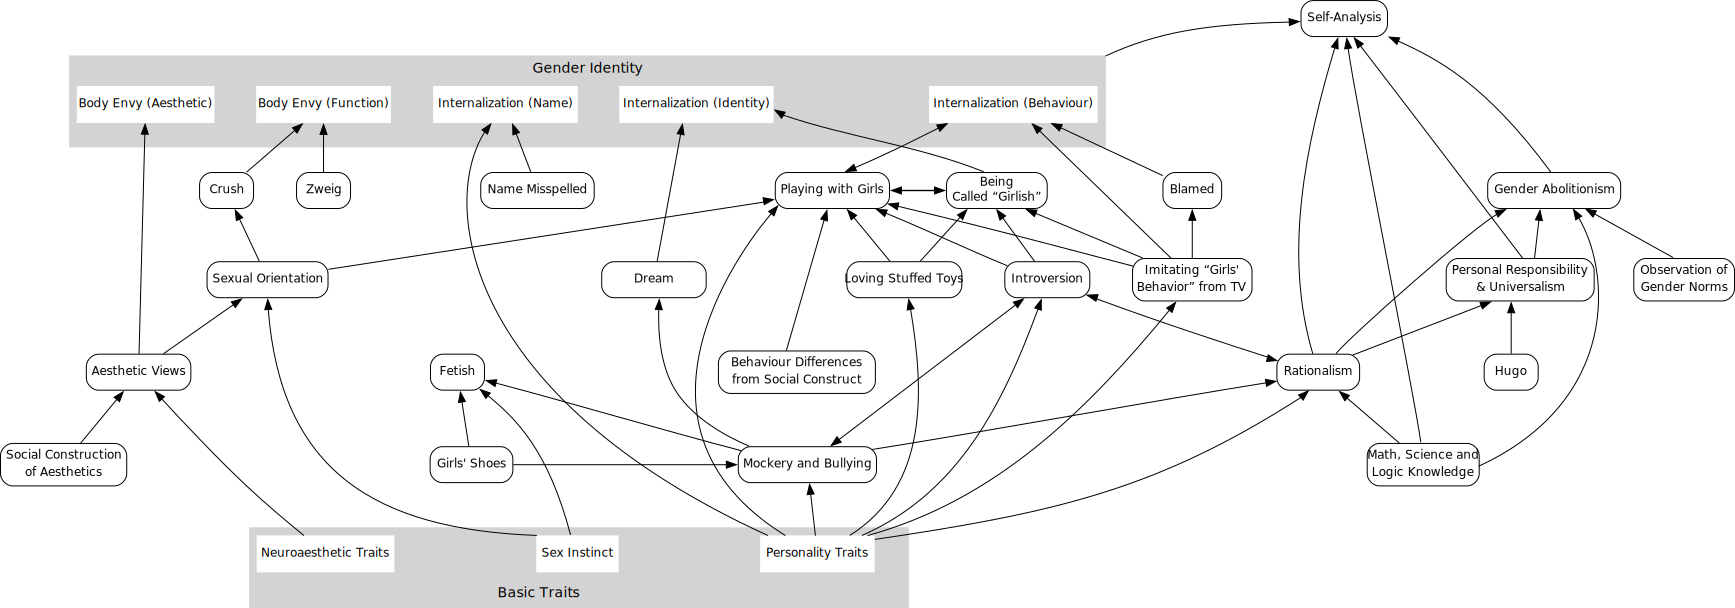
\includegraphics[width=\textwidth]{figures/bundle_of_gender_identity}
    \caption{Origins of the author's gender identity. Visualised using graphviz \parencite{Ellson2001Graphviz} and manually corrected with Inkscape \parencite{Inkscape}.\label{fig:bundle}}
\end{figure}

The ``similarity'' and ``relatedness'' between them is also shaped by society and culture; otherwise, they would be independent and unrelated phenomena. From beginning to end, gender is not inherent in the individual (me), but in the external society. It is the pervasively gendered society and culture that assigns a gender to everything, including our bodies, clothes, behaviours and personalities. The individual, in the interaction with these ``gendered'' things, internalises social norms and develops a so-called ``gender identity.'' Therefore, ``gender identity'' is not an internal attribute but one of many components of our ``narrative identity'', it is the product of the neuroplasticity of our brains. The childhood traumas (e.g., my experience with the shoes) are also an important part that shaped our gender identities, just like they could shape other components in our narrative identities.

% Does a name have a gender? \footnote{Chinese is a language without grammatical gender. } Does a specific colour and style of shoe have a gender? Does encouragement and care from friends have a gender? Does playing with stuffed animals, disliking sports, roughhousing, or covering one's mouth to laugh have a gender? Does a specific geographical space, if not labelled ``Girls' Bathroom,'' have a gender? Does a specific body morphology and aesthetic preference have a gender? Does wanting to establish a relationship with a romantic partner through childbirth have a gender? \footnote{Some might argue that the last two do have a ``gender,'' which involves innate body representation differences. Still, we have already argued that this is a category error. Moreover, even from a biological perspective, a person can have a ``phenotypic female'' body or a uterus and simultaneously produce sperm.}

%Subsequently, I turned to another question: Is my ``gender identity'' really ``female''? This seems to be a Texas Sharpshooter Fallacy. Before I began my analysis, I had presupposed that ``I have a strong sense of identity with female identity and related social symbols.'' However, sometimes I very naturally and automatically think of myself as ``male,'' especially when arguing with trans-exclusionary radical feminists (TERFs) online.

On the other hand, the male components are relatively simple: body representation congruence and the external imposed male socialisation. In particular, there is a representative anecdote worth mentioning. I have a deep aversion to radical ``feminists'' who attack and stigmatise all men. My stance can be traced to Victor Hugo's \textit{Letter to Captain Butler on the Expedition to China} (\textit{L'Expédition de Chine. Au capitaine Butler}), which we learned in middle school language art courses \parencite{Kecheng2007Yuwen}:

\begin{quotation}
    However, I protest, and I thank you for giving me this opportunity. The crimes of the rulers are not the fault of the ruled; governments are sometimes bandits, but the people never are.
    \par Mais je proteste, et je vous remercie de m'en donner l'occasion; les crimes de ceux qui mènent ne sont pas la faute de ceux qui sont menés; les gouvernements sont quelquefois des bandits, les peuples jamais.
\end{quotation}

Compared to a German writer who declared in Hualing Nieh Engle's \textit{Dear Papa and Mama} (亲爱的爸爸妈妈), ``I feel as if it was I who killed those children. We are simply beasts!'', I asked my language arts teacher, why do these two texts contradict each other? If it is as Hugo says, what does the Nazi massacre in Kragujevac have to do with this writer? My teacher said ``it is normal for different writers to have different views on social issues. You can think for yourself whose view is more reasonable, why, and then share your thoughts with me.'' I stood firmly with Hugo's individualist morality. Although this German writer made some seemingly ``profound'' reflections, he essentially still saw himself and the Nazis as ``fellow Germans,'' sharing a transcendental guilt or sin.

While the radical ``feminists'' claimed my anger is because ``you're a man'' and has been ``triggered'' \footnote{急了, \textit{jí le}, a Chinese internet slang for getting flustered or angry when your weak spot is hit.}: ``You think reason is more important than the real suffering of women. This is a thought of male privilege. You fundamentally do not understand our female experience.'' This view is clearly influenced by post-structuralists and feminist philosophers like \textcite{Irigaray1985Subject, Harding1986Science}. While the truth is precisely the opposite: it is because I was arguing with them to defend my ethical principles against irrationality and collective responsibility, and in this process, I was labelled as ``male,'' which shaped the male aspect of my self-identity. If "opposing `feminism' is a male political view" and "I oppose `feminism,'" then maybe I am "male."

Ironically, when debating with extreme nationalists who said that ``all Japanese people are guilty, there is no innocent one under the atomic bomb,'' \footnote{Referring to Hiroshima and Nagasaki.} they claimed that my opinion is "women's kindness." \footnote{妇人之仁, \textit{fù rén zhī rén}, an old Chinese idioms means "excessive tendency to clemency" or being "too soft-hearted" in a pejorative sense.} My opinions on "feminism" and nationalism are almost logically isomorphic: an oppressive power (patriarchy/Japanese militarism) commits evil in the name of a specific group, which does not grant the oppressed group the right to indiscriminately attack the former group in return, because this power clearly did not receive authorisation from the group it claimed to represent. How the same ethic framework is interpreted and what ``gender'' it is assigned depends entirely on the external sociocultural framework, the observer's position, and even an instrumental purpose in a specific context. The interpretation is not based on any objective, consistent standard, but serves the interpreter's own political agenda.

%Thus, this phenomenon not only occurs in childhood but also appears continuously throughout a person's life. It is just that for most people, whether cisgender or transgender, after their gender identity is established, they will consciously resist the invasion from another gender. I happen to not care much about ``gender.'' I don't think my gender identity is very important to me, not my core identity, so I didn't resist it.

More importantly, my reliance on reason is not ``a thought of male privilege.'' In my whole life, every ambiguous or self-contradictory rule serves the power, which is used to degrade or bully me. It is an obscurantism strategy that created unescapable violence. "Reason is a thought of male privilege" is nothing more than the newest of them. My childhood experiences made me feel that the real world is chaotic and painful, while mathematics, logic, and science are orderly and beautiful. I remember very clearly when I was being bullied, how my heart raced, my legs trembled, and tears streamed down my face uncontrollably, while I insisted on telling them, ``You only hit me because your ideas are all unreasonable, because you can't win a debate against me.'' For me, reason has never been masculine. It is intimately intertwined with the most feminine experience of my gender identity. \footnote{I am not saying "reason is a feminine trait," which is another form of gender stereotype. I am saying that my love for reason shares a common origin with the female component of my gender identity.} Reason was the only shield of that little kid in the red shoes in their most vulnerable moment. $2+2=4$ won't become $2+2=5$ just because I "don't look like a boy." No one can arbitrarily change the laws of nature to create an excuse to bully me. In a world full of chaos and pain, it is the only clean, pure, and trustworthy thing. It is my shield, my weapon, my sanctuary. This is the literal meaning of "enlightenment": use the light of reason to lighten all darkness of superstition, privilege, dogmatism, tribalism, and obscurantism.

%It is the same for this self-analysis. I did not ``disrespect'' my subjective experience. On the contrary, I very seriously analysed my subjective experiences, placing them on the same epistemological level as all the knowledge I could obtain from other sources. When I proposed that ``natural selection cannot encode abstract concepts,'' I was not just discussing evolutionary biology and neuroscience. I also recalled the subjective experience of seeing my younger siblings and cousins randomly sucking things as kids, and elders teaching them, ``Don't suck that.'' Our naive knowledge and scientific knowledge are interconnected and mutually shape each other. Respecting experience is not about unconditionally accepting it as a metaphysical truth, but about, as Spinoza did, seriously understanding and analysing, integrating it into one's knowledge network with cross-validating connections with all other knowledge. Far from ``disrespecting subjective experience,'' I have given my subjective experience the highest respect.


%\section{Vertigo}\{sec:vertigo}
%After organising this self-analysis, I looked it over with satisfaction a few times. It was not long before I began to doubt this narrative, because I realised that some things seemed to be just "invented" rather than recalled by me, such as the story of being bullied because of my shoes. I have a memory of wearing red gymnastics shoes in elementary school, and I have a memory of being bullied by bad kids; both vivid and rich. In contrast, the causal relationship is entirely abstract and empty, without detail. I cannot find a memory of "10-year-old me crying and clearly realising that they were bullying me because of my shoes." I cannot even recall realising it at age 12 or 14. Not only that, but I had never seriously thought about why they bullied me before.

On the other hand, I cannot and will not ask them, and they have likely forgotten it entirely -- as we all know, this is typical for bullies. Thus, the truth is, I do not know why they bullied me at all. Perhaps it was simply because I looked easy to bully, or because I was introverted and didn't talk much. I "invented" this causal relationship after setting the goal of "finding the origin of my gender identity" and then recalling and analysing. This is a classic Texas Sharpshooter Fallacy.

In contrast, the memory of being mocked by classmates for wearing red gymnastics shoes is very vivid, specific, and full of detail. A case in point is that once in Chinese class, the teacher asked us to bring some childhood photos and tell stories based on them. In the photo I brought, I was wearing such shoes, and a classmate mocked me, "So you've been wearing girls' shoes since you were a kid" (or something like it), and I angrily snatched the photo back. The causal relationship between them is supported by details. Additionally, I found these childhood photos of me wearing red gymnastics shoes at home. (\cref{fig:shoes})

The story of visiting the museum is similar. The memory of being mocked and heckled by some male classmates, urging me to get down so they could play, and me crying in a corner while enviously watching the girls' group encouraging each other, is very real. The memory of my name being mistyped in childhood is also like this. I remember my mum angrily saying, "Can't they see it is a boy in the photo? Why would they use this character?" and demanding that I go to school the next day and have the teacher change it. This still happens today; many friends who clearly know my legal name, and even government officials, have typed my name as the feminised version. I even found physical evidence, such as name tags or documents. (\cref{fig:2})

Similarly, although I have a vivid memory of lying in bed and recalling the dream. I remember trying to fantasise about the dream's content to find peace and calm to help me sleep during a night of insomnia, the so-called causal chain from "my feet are girls' feet" gradually spreading to "I am a girl" is a "recent invention."

I even began to question those detailed and rich memories, as they could theoretically be retrospectively constructed. I tried to find physical evidence, such as the photos of me wearing red gymnastics shoes and the middle school's name tag with the wrong name. I also found the book \textit{Letter from an Unknown Woman}, which I read as a child, but most of my memories lack such corroborating evidence.

I tried to rationalise the reliability. Although our memories is not 100\% factual, a study by \textcite{Diamond2020Truth} shows that 93--95\% of verifiable details in human memory are accurate. With such a rate, the broad framework of the narrative and the conclusion we reached -- "gender is a product of the individual's interaction with and internalisation of social norms" -- are relatively reliable.

It no longer relies on a single, highly hypothetical causal chain like "being bullied because of the shoes, therefore seeing my feet as 'girls' feet,' and then gradually extending that to 'I am a girl'." Instead, it is based on a social pattern that repeatedly appeared throughout my development, summarised from a large amount of memory data: the individual's neutral personality traits, behaviours, and used items were repeatedly labelled with "gender" by the external social environment, accompanied by strong emotional feedback such as ridicule, discipline, exclusion, and even trauma. This series of interactions shaped the individual's perception of "gender" like a network or a "chain reaction."

After resolving the issue of memory reliability, I turned to another question: Is my "gender identity" \footnote{We will continue to use this term for now, although my definition differs from the mainstream.} really "female"?

This still seems to be a Texas Sharpshooter Fallacy. Before I began my analysis, I had presupposed that "I have a strong sense of identity with female identity and related social symbols." However, sometimes I very naturally and automatically think of myself as "male," especially when arguing with trans-exclusionary radical feminists (TERFs) online.

When they criticise or insult all "phenotypic males" in some gender-essentialist way (e.g., "all men are oppressors"), I feel very angry and use myself as a counterexample to refute them. Of course, this is partly because I know very well that their so-called "men" refers to phenotypic sex, not gender identity. It at least shows that although I usually feel uncomfortable when being called or classified as "male," this discomfort is not greater than my hatred for irrationality. If classifying myself as "male" can provide a valid counterexample to refute their argument. I am happy to substitute myself into $ \text{Male}(x) $ and logically falsify their universal proposition of $ \forall x (\text{Male}(x) \rightarrow P(x)) $.

I am not sure if this counts as a kind of "gender identity." When I argue with TERFs, the structure of the anger is the same as the anger I feel when arguing with extreme nationalists who proclaim that "all Japanese people are guilty, there are no innocent souls under the atomic bomb." \footnote{Referring to Hiroshima and Nagasaki.} I believe my anger is from the irrationality and collective responsibility. These two scenarios are almost logically isomorphic: an oppressive power (patriarchy/Japanese militarism) commits evil in the name of a specific group, which does not grant the oppressed group the right to indiscriminately attack the former group in return, because this power clearly did not receive authorization from the group it claims to represent.

While for me personally, there is a significant difference between these two situations: I am obviously not Japanese, so when I argue with extreme nationalists, I am very clear that this is a purely rational anger against irrationality. In the other situation, because I had not deeply thought about gender identity at the time, and their definition of "male," along with that of the broader society, did include me, the target and direction of this anger were often confused. I sometimes genuinely felt that I was a (specifically defined) "male" and that I was being insulted.

From a particular perspective, this is also "internalising a gender identity through interaction with a pervasively gendered society." TERFs use a crude, essentialist method to impose the label "male" on me. For the sake of debate, I strategically accept this label and develop complex emotional reactions around it. This "contextual male identity" and the "female identity," I feel, in many other scenarios, are formed by the exact same mechanism.

Thus, this phenomenon not only occurs in childhood but also appears continuously throughout a person's life. It is just that for most people, whether cisgender or transgender, after their gender identity is formed, they will consciously resist the invasion from another gender. I happen to not care much about "gender." I don't think my gender identity is very important to me, not my core identity, so I didn't resist it. Ironically, my ignorance of gender has allowed "gender" to be able to freely "invade" my "self." Some other "gender fluid" people may also stem from a similar cognitive mechanism. \footnote{I did not rule out other mechanisms of gender fluid. }

%\subsection{My Philosophy}\label{subsec:my-philosophy}
%I recalled a language arts class in my middle school. This was the source of my opposition to collective responsibility and my earliest philosophical thinking, though I didn't know that ``this was philosophy.'' There were two consecutive texts in my middle school language art textbook: Victor Hugo's \textit{Letter to Captain Butler on the Expedition to China} (\textit{L'Expédition de Chine. Au capitaine Butler}) and Hualing Nieh Engle's \textit{Dear Papa and Mama} (亲爱的爸爸妈妈).

%Previous philosophical thoughts, such as on nationalism, were almost all categorised by me at the time as ``political commentary,'' or political commentary that used scientific (including formal sciences like mathematics) knowledge, like treating the extremist statement ``all Japanese people are guilty'' as a universal proposition and then using Japanese anti-war activists as a counterexample to falsify it. I had never thought that I was thinking about philosophy.

The first text, as its name suggests, is a letter from Hugo to a French captain, criticising the Anglo-French invasion of China. The second text is about a memorial commemoration event of the Nazi massacre in Kragujevac, Yugoslavia. In the event, writers from all over the world discussed ``War and Literature.'' Among them was a West German writer named ``Ming Hebai'' \footnote{``明赫白'' in Chinese. I couldn't find who this person is, what their German name is, or what works they published. It might be a pseudonym created by Hualing to protect them.} who made a statement that I found very confusing:

\begin{quotation}
    The West German writer Ming Hebai slowly stood up. He said gravely, ``\ldots I have a sense of guilt: I feel as if it was I who killed those children. We are simply beasts! All concentration camps must be destroyed! I am very grateful that you allow me to be with you\ldots''
    \par 西德作家明赫白缓缓地站起来,他沉重地说:“……我有犯罪感:感到是我杀害了那些孩子。我们简直就是禽兽!所有集中营都必须粉碎!你们允许我和你们在一起,我非常感激……”
\end{quotation}

I found this passage confusing because of Hugo's article before it, in which Hugo said:

\begin{quotation}
    However, I protest, and I thank you for giving me this opportunity to do so. The crimes of the rulers are not the fault of the ruled; governments may sometimes be robbers, but the people never are.
    \par Mais je proteste, et je vous remercie de m'en donner l'occasion; les crimes de ceux qui mènent ne sont pas la faute de ceux qui sont menés; les gouvernements sont quelquefois des bandits, les peuples jamais.
\end{quotation}

I asked my language arts teacher, why do these two texts contradict each other? If it is as Hugo says, what does the Nazi massacre in Kragujevac have to do with this writer? ``The crimes of the rulers are not the fault of the ruled!'' Hugo did not need to say, ``I feel as if it was I who burned the Old Summer Palace, we are simply beasts.'' That makes no sense.

My teacher said it is normal for different writers to have different views on social issues. You can think for yourself whose view is more reasonable, why, and then share your thoughts with me.

I stood firmly with Hugo: ``The crimes of the rulers are not the fault of the ruled.'' Because the Anglo-French invasion of China was not done by Hugo, and he had no power to stop it, the Kragujevac massacre was not done by Ming Hebai, and he also had no power to stop it. So why should they bear responsibility for things they did not do and could not prevent? Therefore, although Ming Hebai made some seemingly ``profound'' reflections, he essentially still saw himself and the Nazis as ``fellow Germans,'' and his intellectual realm was inferior to Hugo's.

%Then I took the opportunity to criticise some teachers who use collective punishment to maintain classroom discipline. If they couldn't find who was whispering, they would punish all the students in that area. This was not just a classroom opinion, but quickly became a thinking tool for me to understand the world.

At that time, it coincided with the 3/11 earthquake in Japan, and there were some extremist comments on the Chinese internet. I wrote a short story about a Japanese rescue team member who became friends with a Chinese victim of the Wenchuan earthquake when he came to China in 2008. After the 3/11 earthquake, the Chinese person was very worried about their Japanese friend's safety and couldn't contact him. Later, they received an email from the Japanese rescuer's family that he had died in the rescue efforts of the 3/11 earthquake. I found the draft of this story (\cref{fig:notebook}), and I discovered that the story was written from the first-person perspective of a little girl (the victim). Moreover, almost all the fictional stories I wrote at that time were from a girl's first-person perspective. I completely did not notice this issue at the time, and I can find no memory of ever thinking about it.

\begin{figure}[htbp]
    \centering
    \includegraphics[width=0.7\textwidth]{figures/middle_school_notebook}
    \caption{Draft of a short story written by the author in middle school.\label{fig:notebook}}
\end{figure}

This demonstrates that my philosophical views and my gender identity emerged at roughly the same time. They converged after my gender identity became strong enough that I could not ignore, leading me to analyse myself with the intellectual tools that already existed. They may both stem from my childhood experiences. They made me feel that the real world is chaotic and painful, while mathematics, logic, and science is orderly and beautiful. They provided me with a shelter, but this small world is ultimately limited. The external society is still full of irrationality, which drives me to want to completely smash it and rebuild the entire world with mathematics, logic, and science.

This recalls a few small childhood incidents, one of which is that when I was very, very young, I believed that human traffickers did not exist; they were just something my parents made up to scare me. I believed that what I hadn't seen didn't exist. I easily considered it a kind of naive materialism or positivism before I was horrified to realise it was only one step away from subjective idealism.

The statement ``what I haven't seen doesn't exist'' contains two elements:

\begin{enumerate}
    \item ``I'' -- the subject of the judgment.
    \item ``seen'' -- the standard of the judgment.
\end{enumerate}

If I emphasised the ``seen'' and realised that personal ability is limited but still believes in an objectively verifiable physical world, thus extending the subject of ``seen'' from ``I'' to the scientific community or humanity as a whole, and extending ``seen'' to the objective, public ``verifiable,'' one develops towards materialism, positivism, or naturalism. This is the path I took.

If I emphasised the subject ``I,'' and push it to the extreme, the existence of things depends on ``my'' perception, then the entire ``existence'' of things is ``to be perceived.'' Things I cannot perceive do not exist, which leads to subjective idealism.

The thought ``what I haven't seen doesn't exist'' may have been a fork in the road for my personal philosophy. Perhaps the starting points of some completely opposed ideas are much closer than we thought.

Then I realised that my method of analysing the ``non-existence of a complete, ontological gender identity'' is almost identical to \textcite{Hume2007Treatise}'s subjective empiricist argument for the ``non-existence of the self'': I looked inward, saw nothing called ``gender identity,'' only saw many childhood experiences and my reactions to them being artificially grouped together.(\cref{fig:bundle}) The only difference might be that I explained it in a physicalist way as ``reconstructing the training set from the output of a neural network'' and cited scientific research to prove the credibility of memory. \footnote{Hume is considered the precursor of cognitive science, so I was standing on his legacy and reinvented his method.}

\begin{figure}[htbp]
    \centering
    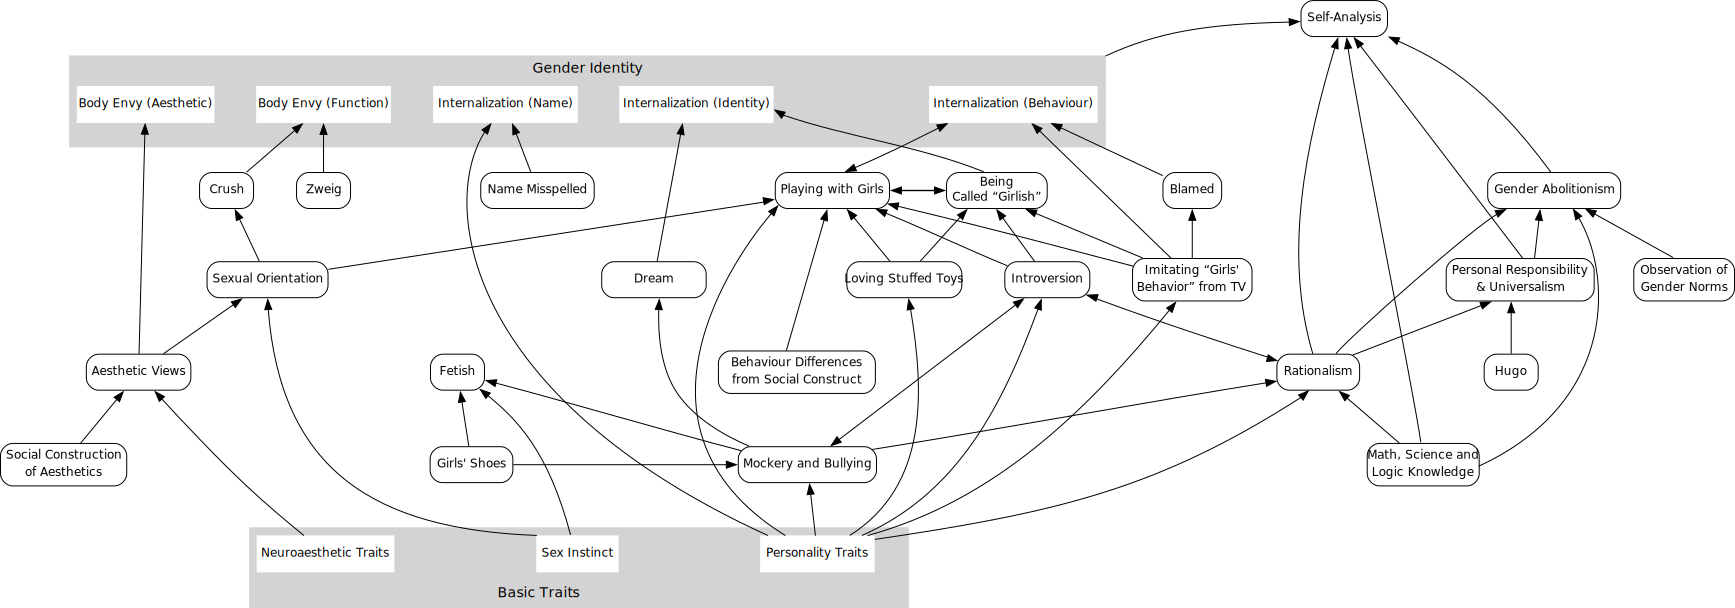
\includegraphics[width=\textwidth]{figures/bundle_of_gender_identity}
    \caption{The author's ``bundle of gender identity,'' like Hume's ``bundle of perceptions.'' Visualised using the Python library graphviz and manually corrected with Inkscape. Due to space and constraint limitations, the neurodermatitis and the events about girls' bathroom are not shown in the diagram.\label{fig:bundle}}
\end{figure}

The second thing is that once, when I was little, I asked my mum, ``Mum, why are you always the one cooking at home? Why doesn't Dad cook?'' My mum said, ``Because Dad is tired of working.'' Then I said, ``You have to work too, aren't you tired?'' My mum was very happy, saying I had grown up and cared for my mum. However, at that time I didn't know what was caring. I just found a logical flaw, which meant that the initial reason was either false, incomplete, or the entire system was built on an unfair double standard. A very similar incident was when I was visiting relatives as a child and questioned the division of kinship terms in our local dialect. I asked my parents why there are more precise terminologies for paternal relatives than for maternal relatives, and they responded with ``it's tradition, don't ask stupid questions.''

%Many years later, I learned that this was precisely the ``categorical imperative'' proposed by Kant centuries ago: only follow the maxim that could become a universal law. The young me discovered that my mum's reason, ``if you're tired from work, you don't have to cook,'' could not become a universal law, otherwise nobody would cook, and we will be starved to death, no rational person would will such a world. This meant that the initial reason was either false, incomplete, or the entire system was built on an unfair double standard. \footnote{I support Kant's ethics but not the transcendental idealism. I had tried to abandon Kant's metaphysics and rebuild the normative part of his ethics in a physicalism worldview, which seemed very difficult, and I ultimately did not complete it. }

%The true, unstated maxim was likely not about tiredness at all, but about socially prescribed gender roles. The actual operating principle might have been something like: ``The woman in the household is responsible for cooking, regardless of her tiredness.'' When subjected to the categorical imperative, this maxim also fails. A rational being cannot will a universal law that assigns duties based on arbitrary characteristics like gender rather than on a fair, impartial, and rational distribution of labor. Such a law would treat certain rational agents merely as a means to get food, which violates Kant's second formulation of the categorical imperative, the Formula of Humanity.

% my mother's brothers and male cousins were all ``jiù'' (舅), and her sisters and female cousins were all ``yí'' (姨). My father's sisters and female cousins were all ``gū'' (姑). In contrast, my father's brothers and male cousins were divided into three categories: elder brother and male cousins were ``dàyé'' (大爷), younger brother and male paternal cousins were ``dàda'' (大大), and younger maternal male cousins were ``biǎoshū'' (表叔)

These memories led me to examine a more fundamental question: where does my obsessive need for systematicity and logical consistency come from? Is it merely an acquired academic habit, or does it have deeper roots? In the process of exploring my ``gender identity,'' I unexpectedly found a possible answer. Research on atypical gender experiences is sometimes associated with autism spectrum disorder (ASD). Initially, I did not associate this with myself, but these cognitive traits, like analytical understanding, systematic thinking, and problems in understanding social norms, highly resemble my experience.

I started to consider the possibility that I might have ASD or a subclinical Broader Autism Phenotype (BAP). As a self-test, I scored 36 in the Cambridge Autism-Spectrum Quotient \parencite{BaronCohen2001Autism}. Although this result cannot be used as a diagnosis, it can be used as a heuristic explanatory framework for understanding myself. Of course, my case might not be typical: autistic individuals usually have a strong interest in a specific area, whereas my interest is almost in the entire world.

It should be noted that this does not constitute a biological determinism, and does not overturn my previous hypotheses about the origin of my preference for science and logic. The ``special interests'' of autistic individuals are remarkably diverse, and everyone's ``special interest'' is also formed through interaction with society. An autistic child cannot innately know what a dinosaur or a train is. The main reason for my ``interest'' is still likely due to a deep hatred of the illogical real world. Without this experience, my ``special interest'' might also be a specific field. My experience of order in science and logic and the subsequent willingness to rebuild the entire world are not an inevitable result of autism, but my own agential choice. The biological determinist assumption that my love for reason and science was directly originated from the autistic traits is absurd because it is somewhat implying that all scientists and philosophers are autists.

This discovery also provided new evidence for my view that ``neutral innate neural traits are assigned gender labels by society and culture.'' In the research I read on ASD (including previous Asperger's syndrome), there were two papers on FtM or FtX individuals who said they felt not like females or were more like males since childhood. One paper's author followed Dr Hans Asperger's original view from his 1944 description, that ``the autistic personality is an extreme variant of male intelligence,'' and considered the neurological traits of autism to be a so-called ``male brain'' \parencite{Kourti2019Dont, Kraemer2005Comorbidity}.

However, my own situation is more complex. As a child, I disliked socialising and preferred to read and think alone. I was told by elders that I was like a little girl and was bullied by classmates. This is the exact opposite of Dr Hans Asperger's classic explanation. Yet, as an adult, I am considered ``very masculine'' because of my logical thinking style, and some TERFs have claimed that ``your way of thinking is male, you don't understand our female experience at all.'' The biological basis is neutral. How it is interpreted by society and culture, how this interpretation acts on an individual, and what kind of self-identity the individual ultimately forms are largely arbitrary. Without society and culture, it is just a neurological trait that has nothing to do with ``gender.''

How it is interpreted and what ``gender'' it is assigned depends entirely on the external sociocultural framework, the observer's position, and even an instrumental purpose in a specific context -- whether it is describing a quiet child with a ``good'' faith or attacking a debate opponent with a bad faith. The interpretation is not based on any objective, consistent standard, but serves the interpreter's own agenda.

%\section{Philosophical Critique of Gender Identity}\label{sec:philosophical-critique}
%%As we said above, if we apply the standards of Aves to Mammalia, we will conclude that almost all humans are intersex. However, in the following argument, let's not jump to such a radical stage.

%Let's first achieve a kind of logical consistency within humanity: individuals with gynaecomastia are intersex. This is the necessary result of applying the standard of breasts as part of ``phenotypic sex'' from other domains to the domain of ``intersex.''

%Then, according to the old diagnostic criteria, like in ICD-10~\parencite{WHO1992ICD10} or DSM-IV-TR~\parencite{APA2000DSM4}, an individual with gynaecomastia who self-identifies as male should be considered a specific kind of transsexual (XtM), because they have ``a sense of discomfort with their anatomic sex,'' and want to make it ``as congruent as possible with one's preferred sex.'' The medical treatment should also be considered ``gender affirming surgery.'' Ironically, both diagnostic criteria explicitly exclude intersex individuals, which is extremely hard to understand.

%However, rather than achieving greater inclusivity by including intersex people, the editors continue to maintain a \textit{de facto} exclusion of intersex people by introducing the concept of  ``assigned sex at birth''~\parencite{APA2013DSM5, WHO2019ICD11}. Not only individuals with gynaecomastia were excluded from transgender, but many traditionally defined

The preceding biological analysis established that ``gender identity'' is not an innate, immutable essence housed within the brain or soul, but rather a product of neuroplasticity formed as the brain ``overfits'' to a noisy and arbitrary social norms. Consequently, because the biological hardware is merely processing the software of culture, I shift the focus from the biological mechanism to the philosophical structure of the social constructs themselves. I will demonstrate that the contemporary theoretical framework surrounding gender -- specifically the dichotomy of ``cisgender'' and ``transgender'' and the concept of ``assigned sex at birth'' (ASAB) -- is full of internal contradictions to maintain a precarious ideological order.

Let us have a thought experiment: an intersex child is assigned female at birth, but gets lost at a very young age, is reassigned male by adoptive parents, and is raised as a boy. After adulthood, their body is closer to a ``phenotypic male,'' but their gender identity is female. According to the definition of \textcite{APA2013DSM5, WHO2019ICD11}, this individual is a ``cisgender female.''

By introducing the concept of  ``assigned sex at birth,'' some intersex people are excluded from transgender. Ironically, if we use ``phenotypic sex'' to define transgender people, we can capture this individual's unique gender socialisation experience (XtF) very well. Since the so-called ``assigned sex'' is almost always binary in actual medical practice, it simplifies the patterns of children's gender socialisation using two typical phenotypic sexes, replicating the power framework it seeks to oppose, and in fact, brings back the ghost of gender binary.

When we examine ASAB more furtherly, we will inevitably ask: Is ``assigned sex/gender at birth'' \footnote{In English, both ``assigned sex'' and ``assigned gender'' are used. } a kind of ``sex'' or ``gender?'' What is the relationship between ASAB and gender identity? If gender is unrelated to phenotypic sex and gender identity is not identifying with sex, then logically, being phenotypic or assigned male/female and identifying as male/female are two or three unrelated things. They just share the words ``male/female,'' like the ecological and sociological ``community.''

Therefore, everyone's phenotypic sex (a series of biological characteristics, although artificially selected) or ASAB (a label on a legal document) is ``inconsistent'' with their gender identity (a psychological state). Or more accurately, it is impossible to discuss whether they are ``consistent'' or ``inconsistent.''. Because they describe three essentially different kinds of things, just as we would not say that the social ``community'' a person belongs to is ``consistent'' with the ecological ``community'' they inhabitants.

Conversely, if those whose ASAB use the same word as their gender identity are called ``cisgender,'' and their phenotypic sex or ASAB is ``consistent'' with their gender identity, this means that phenotypic sex and gender are related in some way. Their view on the relationship between sex and gender is not a rigorous philosophical nominalism, but a vulgarised, selectively applied nominalist fallacy. When they need to separate the body from identity, they use nominalism; when they need to establish the cisgender/transgender binary opposition, they secretly retreat to an unreflective realist position.

The conflict between ``nominalism'' and ``realism'' occurs not only between ASAB and gender identity, but also within ``gender identity'' itself: is the ``woman'' of feminism and the ``woman'' of patriarchy the same concept? The ``woman'' who supports feminism and the traditional ``woman'' both self-identify as ``woman.'' Are their gender identities the same? They claim that all people who identify as ``woman'' share some real, existing ``essence'' called ``female identity'', no matter how different their political stances, lifestyles, and values are. And it uses realist labels like ``cisgender/transgender'' to classify these completely unrelated self-identities as the same kind, simply because their name is or is not consistent with their birth certificate.

Moreover, the cisgender/transgender binary opposition fundamentally violates the ``principle of self-identification,'' because it is equivalent to assigning a gender identity that is ``consistent'' with the ASAB to all people who have not explicitly identified as a different one. Most ``cisgender'' people have never made such a statement, nor have they ever been asked ``What is your gender identity?'' This act is almost completely isomorphic to the ASAB; both are top-down, external assignments without consent. A movement, whose important ethical principle is ``opposing non-consensual identity assignment,'' \footnote{\textcite{Butler2025Who}: \ldots Can we decide what being or having a sex means outside of a framework that establishes and reestablishes sex, that is, a framework that has to be imposed with regularity through time, one where the power to self-assign is exercised by those who have already \textit{been} assigned? Some trans people turn against all assignment, claiming that it invariably works in the service of hierarchy.} relies on the non-consensual identity assignment of most people. It repeats the oppressive structure it criticises, but only packaging itself in a ``critical'' language.

It implicitly introduces an \textit{a priori} assumption that ``everyone has a gender identity,'' because the definition of ``cisgender/transgender'' depends on the existence of it and its ``consistency'' with ASAB. By establishing a classification based on ``gender identity,'' it made ``having a gender identity'' a necessary condition for being a complete-socialised person. If you are not ``transgender,'' then you must be ``cisgender'' -- humans are deprived of the options ``I don't have this thing at all,'' ``null,'' or ``undefined.'' Under this framework, the position of ``I have no gender identity'' becomes invisible or politically incorrect. Individuals are deprived of the right to ``quit the game''; they are either ``cisgender'' or ``transgender.''
%\footnote{This topic reminds me that I once intended to declare my gender identity as null. I was using it in a very sincere, technical sense (value unassigned). Nevertheless, I immediately realised that I cannot express it like how a computer handles null. When someone asks about my gender identity, I cannot directly throw a ``NullPointerException: field \`gender\` not found in object \`user\`'' in their brains. In real life, it is still a textual label. The ``null'' I am writing in this article is four Latin letters, not the technical null.}

Most fatally, when they set ``cisgender'' as a synonym for ``non-transgender'' or ``having not stated their gender identity,'' they are saying that all transgender people are cisgender at birth. This is equivalent to saying that ``transgender people were cisgender and changed for specific reasons,'' which becomes the conservative viewpoint. This flaw is logically and politically devastating.

%``Transgender'' is also this kind of imposed identity if we view it from a specific perspective. Some activists and scholars like \textcite{Arraiza2024After} argue that neurological markers are ``biological determinism'' and strip trans people of their rights. However, if we completely abandon neurological markers, it is effectively saying a person must participate in the social gender construct and have a ``gender identity'' to get medical treatment. People are striped the right of refusing to participate in gender constructs and identity politics, and just going to a doctor and say, ``I have a persistent rejection of this part, it affects my life, and I want to remove it to resolve my suffering.'' The only reason this isn't the primary path is that the ``gender identity'' narrative currently has more followers.


%\section{For Abolition}\label{sec:for-abolition}
%Critics might accuse me, ``your theory is just a wrap of queer theory with analytic and scientific languages.'' I admit that my model is similar with \posscite{Butler1990Gender} theory in some senses, including denying a Cartesian self and supporting a constructed/shaped self-consciousness by the external environment through discursive effect/neuroplasticity. The most significant difference lies in our ontological premise: I believe in an objective reality that exists independently of the human mind \footnote{I admit that it may sound like begging the question, but obviously it's off-topic to provide a sophisticated argument for scientific realism here. }; and for queer theory, our understanding of reality is constructed through discourse and we cannot perceive it without mediation. In most contexts, ontology might be nothing more than a boring metaphysical intellectual game. While in this case, ontology is everything, it decides two completely different strategy.

From a scientific realistic aspect, gender shapes our understanding about the biological, psychological and sociological diversity of human beings, which is inconsistent with its real mathematical structure. This misunderstanding, also known as ``stereotype,'' affects our self-identity. Being analogous to deep learning (connectionism), gender construct is a corrupted training data that contains two flawed classes: Class 0 (female) is consisted of feminine faces, vaginas, clitorises, developed breasts, pink, purple, brooms, mops, kitchens, dolls, stuffed toys, dresses, Mary Jane shoes, jewellery, make-up \ldots~On the contrary, class 1 (male) is made up of masculine faces, penises, testicles, undeveloped breasts, Adam's apples, beards, blue, computers, documents, architecture, toy cars, pants, suits, ties \ldots~An individual's gender identity is the product of it. ``Gender identity'' is our brains desperately trying to find a pattern in a chaotic, nonsensical, and wrongly labelled set of social data. It latches onto these arbitrary connections and creates a rigid internal model that doesn't actually reflect a fundamental reality.

Therefore, the most fundamental ``-centrism'' in our society is not androcentrism, heterocentrism, or cisgender-centrism, but gender-centrism -- an ideology that establishes ``gender'' as the core category for understanding the world and ourselves. By assigning a gender to everything, ``gender'' attempts to bring the entire world under its dominion, to establish itself as the centre of the way humans perceive the world. It prevents humans from accurately perceiving the real mathematical structure of the world. The gender-centrism is so ancient, so deep, that even the most so-called ``liberatory'' theories or social movements -- feminism or LGBTQ -- have not escaped it or do not dare to escape it. They merely try to change cells within the prison. They resist the ``oppression of gender,'' but they are afraid, unwilling, unable, or refuse to resist the existence of ``gender'' itself.

For other socially constructed identities, such as nation, race, class, profession, etc., their supporters clearly know that these identities are socially constructed. Only gender, a completely externally imposed system, is regarded by the entire political spectrum as something \textit{a priori} and essential. The only disagreement is where this essence lies -- in our genitals (``scientific'' gender essentialism), brains (transgender mechanistic materialism), or souls (transgender idealism and religious conservative). It is even regarded by some groups as the ``true self,'' a symbol of ``freedom and empowerment.''

``Gender essence'' or ``gender identity'' is proclaimed by all political camps to be innate, internal, profound, and constitutive of essence, yet it is clearly acquired, social, superficial, and shaped by society and culture. It defines our essence, governs our entire lives, is assigned before the formation of the self identity, and claims to be the self itself. It simultaneously occupies the domains of science, humanities, politics, and religions. \footnote{The ``religion'' refers to the conservative narrative of ``the two sexes are the natural order created by God'' and the liberal narrative of ``a soul born in the wrong body.''} It has a unique, unquestionable, cross-political-spectrum ontological privilege.

% To declare a specific one as our ``core'' self is a questionable assumption. It suppresses the expression of other types of self-identity. The dominant status of ``gender'' over other personality traits and self-identities also reduces the culturally and socially available combinations, leading to a decrease in the freedom of self-expression.

Since the real problem lies in an omni-encompassing ideology that attempts to assign ``gender'' to everything, the most fundamental solution is to abolish the whole gender construct. I hereby propose a solution aiming at abolishing gender by strictly limiting ``sex'' and ``gender'' to atomic entity, detaching them from individuals.

% (\cref{tab:1})
%
%\begin{table}[bt]
%    \caption{Comparison of the Claims and Realities of Gender.}
%    \label{tab:1}
%    % Use "S" column identifier to align on decimal point
%    \begin{tabularx}{\textwidth}{l X X}
%    \toprule
%    Characteristic & Claim          & Reality     \\
%    \midrule
%    Time	& Innate, before self-awareness	& Acquired after learning \\
%    Source	& Internal, in our brains, genitals or souls	& Internalised from society and culture \\
%    Hierarchy	& Profound, equivalent to self-perception	& Superficial, merely a descriptive tool \\
%    Function	& Constitutive of essence, defining existence	& Alienating, psychological colonisation \\
%    Ontological Status	& Cross-political-spectrum ontological privilege	& Arbitrary symbols of language and culture \\
%    Domain	& Science + Humanities + Politics + Religions	& An accidental product of history and culture \\
%    \bottomrule
%    \end{tabularx}
%\end{table}

%Concepts like ``sexual orientation,'' ``gender identity,'' and ``intersex'' were not created to ``liberate humanity from gender binary,'' but to ``protect gender binary from humanity.'' They are just a series of ``epicycles.'' Like the pre-Copernican astronomers, our modern psychologists and sociologists are creating these epicycles for those who do not conform to the norm (homosexuals, bisexuals, transgender people, intersex people). In this way, the system can safely isolate them as ``exceptions,'' thus maintaining the Ptolemaic model (the cisgender heterosexual endosex binary norm) in most situations. The true purpose of historical ``epicycles'' was not to ``help planets find their true orbits,'' but to avoid a radical paradigm shift.
%Otherwise, as we discussed earlier, why does a change intended to increase ``inclusivity'' -- using ``assigned sex'' instead of ``phenotypic sex'' in the definition of transgender -- logically reduce inclusivity and the scope of people who can be considered ``transgender''?
%
%Some zoologists call non-human animal individuals ``gender non-conforming'' (GNC) because their behaviour does not conform to the statistical typic for their own ``phenotypic sex'', such as the female chimpanzee Donna, who occupied territory and fought. Primatologist Frans de Waal even claimed that ``primates are born with a gender identity''~\parencite{DeWaal2022Different, Morin2022Frans}. This is effectively saying that gender is a behavioural characteristic of animals, thereby reducing sociology and psychology to a branch of ethology that specifically studies the species \textit{Homo sapiens}, thus making gender a part of sex.
%
%Thus, if we strictly follow this framework, considering the inaccessibility of subjective experience, ``gender identity'' should be regarded as ``using the vocal cords to produce encoded mechanical waves, or using visual symbols created by the species itself to express oneself as male/female.'' It is a behavioural sexual dimorphism of \textit{Homo sapiens}, which is obviously absurd.
%
%Similarly, under this definition, the sex of sexually monomorphic organisms cannot be determined without dissection. The so-called ``male/female'' that is generally judged based on behavioural characteristics should logically be gender, not sex. A case in point is that many lovebird owners judge their pet birds' ``sex'' based on their behaviour, such as incubation, nest building, and position during mating.
%
%If animal behaviour is gender, then botanists describing the reproductive function of a plant as \textit{gender} is a natural extension of the former. The claim by some transgender activists or the biologists who support them that using the word \textit{gender} to describe plants ``harms'' transgender people~\parencite{Oberle2023Benefits} is baseless. The same word, when used for humans, is a political and human rights issue; when used for great apes, it ``proves the naturalness of transgender''; but when used for plants, it becomes a form of ``harm.'' What is the reason for this distinction? This is essentially anthropocentrism, taxonomic chauvinism, and an act of granting our closest relatives the title of ``honorary humans.''
%
%Moreover, even if we analyse it under the mainstream theory, gender is a sociocultural construct, while gender identity is an individual's internal psychological state. These are two different concepts. ``Society'' and ``culture'' cannot be the object of harm. Claiming that the borrowing of an abstract sociological concept, \textit{gender}, will ``harm'' humans who possess an internal psychological state, \textit{gender identity}, is a category error.
%
%Considering that:
%
%\begin{enumerate}
%    \item Sex is not a natural kind, but a social construct, therefore a part of gender.
%    \item Gender is a behavioural characteristic of animals, therefore a biological attribute.
%\end{enumerate}
%
%Therefore: $ S \subseteq G \wedge G \subseteq S \Rightarrow S = G $
%
%QED\@.
%
%It is clearly demonstrated that no one really knows what the difference between sex and gender is. No one really knows what they are talking about. Different activists and scholars, according to their political needs, arbitrarily borrow concepts from other disciplines and redefine them, completely ignoring whether these acts will cause the entire gender discourse system to collapse logically.
%

The biological sex should be strictly confined to the gametes \parencite{Lehtonen2014Gamete, Goymann2023Biological, Hurst1996There, Griffiths2025Biology}. It is related to, and only to, gametes. Individuals do not have such a sex. Sexual dimorphism is a dynamic spectrum that constantly changes throughout evolutionary history. The so-called ``phenotypic sex'' should be dismantled into a series of discrete, decentralised phenotypic traits such as chromosomes, hormones, as well as all morphology and anatomical traits. They are distributed on the sexual dimorphism spectrum, along with sexually dimorphic traits not traditionally classified as ``phenotypic sex'', like height, weight, body hair, and body fat percentage \parencite{Wells2007Sexual}. Individuals do not have an innate gender; they merely ``possess'' gametes, ``live in''  a society and ``internalise'' the culture.
%The imprecise concept of intersex should be replaced by more detailed terms like intergonadal, intergenital, and sexual intermorphism. Gender should be strictly treated as a sociocultural phenomenon.

By biologically confining sex strictly to an unobservable trait, it cannot be ``assigned'' or ``inferred.'' \textcite{Parvin1982Ovulation} reported a person who was completely ``phenotypic male'' and had fathered a daughter, but one of their two ``testicles'' was actually a pure ovary (not an ovotestis), and dissection showed it had previously ovulated. Therefore, most people, even those who have had children, cannot know for sure if they are capable of producing two types of gametes. This makes it lose any possibility of being used for social classification, discipline, and oppression. It becomes a technical term of reproductive biology, completely ``exiled'' from everyday language and the operation of power.

My proposal is completely different from conservatives, who claim to adopt gametic definition, but still rely on the genital in practice, which is self-contradictory. This even includes some conservative scientists, like \textcite{Sokal2024Sex}, who claim that sex is an ``objective biological reality,'' ``determined at conception and observed at birth.'' I agree that sex \textit{sensu stricto} is a objective biological reality, and is strictly binary in Vertebrata. While according to \textcite{Jones2006Gamete}, ``Conception occurs when a sperm and an ovum fuse to become a zygote.'' ``The process of fertilisation, or conception, involves fusion of the nucleus of a male gamete (sperm) and a female gamete (ovum) to form a new individual.'' At ``conception'' (fertilisation), it is just a zygote, a single cell. It has neither sex \textit{sensu stricto} because it cannot produce its own gametes, nor does it have phenotypic sex by lacking a developed body. Even if its genome will guide it to develop into a typical phenotypic male or female under normal conditions, it will not necessarily be so. For instance, if a 46, XY zygote loses its Y chromosome during the first mitotic division after fertilisation, it will develop into a 45, X0/46, XY chimaera (mixed gonadal dysgenesis) or a 45, X0 individual with Turner syndrome \parencite{Gravholt2017Clinical, Jacobs1997Turner, Lopes2014Mosaicism}.

The binaric sex is still a very useful model in evolutionary biology, ethology, and reproductive ecology. It is obviously technically and ethically impossible to capture and dissect all individual animals to examine the gametes they produce. In these cases, researchers should state in their \textit{Materials and Methods} section what proxy they used to estimate the gamete production capacity and the reliability, such as the situation in birds revealed by \textcite{Hall2025Prevalence}. Sex \textit{sensu stricto} itself is a microscopic reproductive biological trait, not an externally observable morphological character.

%\textcite{Polderman2018Biological} claimed that the heritability of gender identity is 30--60\% and consistent with other behavioural and personality traits, which is a category error. As we have said before, ``gender identity'' cannot be encoded in the genome (this would require extraordinary evidence). We can only have a series of genes related to personality traits, cognitive styles, and body representation. Studying the ``heritability of gender identity'' is a huge logical leap. The correct scientific questions should not be: ``What is the biological basis of gender identity?'' but rather: ``Which heritable biological traits are assigned gender meaning by society and culture?'' (sociology). ``How does the meaning interact with the individual to construct a specific gender identity?'' (psychology). ``What is the biological basis of these traits?'' (genetics and neuroscience). Autism spectrum disorder is also highly heritable \parencite{Sandin2017Heritability}, and autistic traits are higher in those working in STEM fields \parencite{Ruzich2015Sex}. Following \posscite{Polderman2018Biological} methods, we might also be able to calculate a mathematically reasonable number of ``heritability of STEM ability'', which everyone would consider an absurd study. Autistic neurological traits are heritable, while participating in STEM fields is an extremely complex result of innate neurological traits, personal experience, academic training and so on. Biological studies of ``gender identity'' are precisely the 21st-century replication of ``scientific'' racism.

At the social level, all gender concepts and any social constructs should be abolished. The biological characteristics previously considered ``phenotypic sex'' should have no more social significance than height or weight. All mention of gender in laws and regulations should be removed. In cases not involving a relationship, replace "man" or "woman" with "person." In cases involving a relationship (such as marriage), replace them with "one person" and "the other person." Gendered pronouns and titles should be abolished, sexual orientation should be considered mating preferences or aesthetic preferences, gender incongruence should be considered a form of body representation incongruent, and gender-affirming surgery should be considered a form of cosmetic surgery. A person's desire to change their body, whether because of innate body representation incongruence or any acquired factor, is a matter of pure personal freedom. These are merely mechanical modifications to our body, its legitimacy stems from bodily autonomy. It does not need an unprovable ``gender identity'' to justify it. Gender markers should be removed from all nonmedical records, and sex markers in medical records should be multi-level (chromosomes, reproductive organs, fertility, hormone levels, etc.) rather than just male/female. All gender-segregated facilities should be eliminated. Clothing stores should no longer be divided into ``men's/women's'' sections, but organised by clothing type (tops, pants, outerwear) and size/fit. Toys should no longer be divided into ``boys'/girls','' but by function and type (e.g., building blocks, dolls, science experiments, art creation) and appropriate age.

Most importantly, ``gender identity'' should be understood literally, ``identity with a gender,'' which is shaped in one's interaction with and internalisation of social gender constructs. The psychotherapist should play the role of a philosophy and science teacher, promoting self-understanding in clients who are exploring their gender identity through Socratic dialogue. It's not about providing answers; it's about providing tools for thinking and empowering the individual to find their own answers. They are rational beings capable of and deserving of a deep, philosophical engagement with their own identity.

We have no need at all to shy away from ``gender identity is the internalisation of social gender norms and gender stereotypes.'' The gender identity of cisgender people is also the internalisation of gender norms and stereotypes. However, it is politically not important. Why is it a virtue when childhood trauma causes a person to have a strong heart, but when it causes a person to develop an incongruent gender identity, it needs to be ``converted?'' This conservative logic is very easy to refute. What should be emphasised is: gender identity is an acquired psychological state, but it is acquired subtly and unconsciously, like the first language. For the person themselves, it feels very "innate." This is how our brains work, it does not mean that we should blame people for "internalising gender stereotypes."

%This transforms the issue from a special identity under identity politics, a special psychological state (identity), and a specific phenomenon, to the dismantling of an oppressive system. Everyone, whether ``cisgender'' or ``transgender,'' is a victim of this system. It is a political issue that requires the participation of the entire society: why do bathrooms need to be segregated by gender, and why do documents need to be marked with gender?



%\section{Dialogues}\label{sec:dialogues}

%\subsection{Dialogue with Gender pluralism}\label{subsec:dialogue-with-gender-pluralism}
%\input{chapters/dialogue-with-pluralism}

%\subsection{Dialogue with Queer Theory}\label{subsec:dialogue-with-queer-theory}
%Critics might oppose my previous statement that ``neither feminism nor LGBTQ has opposed gender-centrism,'' claiming that ``queer theory is against gender-centrism.'' I admit that queer theory is ontologically anti-gender-centric, as argued by \textcite{Butler1990Gender} that they do not consider ``sex'' (phenotypic sex) or gender to be natural, real or stable. Still, there is a huge difference between ontology and methodology.

\textcite{Butler1990Gender} advocated for a strategy of ``repeating'':

\begin{quotation}
    The task is not whether to repeat, but how to repeat, or, indeed, to repeat and, through a radical multiplexing of gender, to displace the very gender norms that enable the repetition itself.
\end{quotation}

The issue is neither whether to repeat nor how to repeat, but what to repeat. For example, it is a kind of ``repeat'' to create a lot of neopronouns, however, this is precisely because of the gendered pronouns in English. Nobody would create a lot of neoterms about bicycles, because there are no masculine and feminine forms of it. This strategy recognises the gender norm's power to define the area and boundary of the battlefield. Therefore, queer theory is ontologically anti-gender-centric yet methodologically extremely gender-centric.

The intended outcome of this strategy was to ``displace the very gender norms'' by showing their constructed and unstable nature. However, as the actual outcome, by constantly talking about and analysing gender, by ``repeating'' gender inside the boundary, it has reinforced ``gender'' as the central issue for understanding ourselves and society. ``Gender'' was originally just an external sociocultural construct, but it is now frequently used as a synonym of ``gender identity,'' an internal psychological phenomenon. \textcite{Oberle2023Benefits} is a typical case, they argued that using the word \textit{gender} to describe plants ``harms'' transgender people. It is an obvious category error to claim that the borrowing of an abstract sociological concept, \textit{gender}, will ``harm'' humans who possess a psychological phenomenon, \textit{gender identity}.

%Every new identity they create is a new ``true self'' that individuals can choose. This makes the most fundamental rule, ``you must have a gender identity'', more unquestionable. The queer theory theoretically opposes the identity politics, yet its strategy seems to offer infinite choices of identities.
Queer theory's strategy created a powerful cultural incentive: to treat all kinds of unconventional personal experiences and identities as a ``gender'', because it has made ``gender'' the most attractive ``liberative'' discourse. If ``gender'' were still strictly understood as a sociocultural construct, xenogender people would likely not see their ``identity'' as a ``gender identity.'' They do so because ``gender'' is currently the most prominent and available discourse of resistance. This paradoxically expands the category of gender to encompass phenomena that might otherwise have been understood in different categories (e.g., as personality, philosophy, or simply as radical individuality). Within the xenogender community, there is already reflection on this issue, and the alternative term xenoidentity has been proposed for those who have similar identities but are unwilling to classify it as a ``gender identity.''

Queer theory's strategy was to engage gender norms on the ``battlefield'' which was defined by itself. The unintended consequence of this engagement was that the battlefield itself -- the very concept of ``gender'' -- became more central, omni-encompassing, and ideologically powerful than ever before, attracting everyone to join it. The strategy recognised the prison's power to define its walls, and sought to ``destabilise'' them by painting them many different colours, but not destroy and escape from it. The outcome was that the ``colourful and comfortable'' prison became more fundamentally entrenched, attracted more and more people to move in and reinforcing the core idea that one must be a prisoner.

%If the gender system cannot accommodate our existence, shouldn't we completely smash this system? Why must we tell them, ``Actually, we are also a kind of `gender'?'' By saying ``we are also a kind of `gender','' they have accepted that ``gender'' is a valuable category worth joining, which gave up the fundamental right to ask, ``Can we abolish the social norm centred on `gender'?'' \textcite{Butler2025Who} is a typical figure of this reformist ideology:
%
%\begin{quotation}
%    The critique of the gender binary, for instance, did not claim that ``women'' and ``men'' are over and done with. On the contrary, it asked why gender is organized that way and not in some other way. It was also a way of imagining living otherwise. The critique of the gender binary turned out to give rise to a proliferation of genders beyond the established binary versions -- and beyond the gender hierarchy that feminism rightly opposes.
%\end{quotation}

As I previously argued, this is precisely because of the ontology of post-structuralism. They do not believe that objective knowledge of the external world is possible. Therefore, the goal is not to match an external truth, but to play with, subvert, and reconfigure the discourses we live within. In contrast, an objective understand of the reality is possible and desirable in scientific realism, which provides an unshakeable foothold for scientific and philosophical criticism and political resistance. The concept of ``gender'' causes most people's perception of the world to be inconsistent with this external, objective reality. The highest goodness and truth is about aligning our internal models with external reality. Gender is a buggy model that creates a mismatch, so it must be abolished. This is a concise demonstration of the fundamental, irreconcilable gap between the scientific worldview of Enlightenment and the post-structuralist one.

%As \textcite{Marx1977Critique} said in his \textit{A Contribution to the Critique of Hegel's Philosophy of Right}:
%
%\begin{quotation}
%    Luther, we grant, overcame bondage out of \textit{devotion} by replacing it by bondage out of \textit{conviction}. He shattered faith in authority because he restored the authority of faith. He turned priests into laymen because he turned laymen into priests. He freed man from outer religiosity because he made religiosity the inner man. He freed the body from chains because he enchained the heart.
%\end{quotation}
%
%The concept of ``gender identity'' leads individuals to equate a social construct with their true self, to internalise an external social construct as a core part of their self. It freed the body from ``gender'' because it enchained the heart. It successfully achieved what classical gender theory could not do for thousands of years.

In an interview with \textcite{Williams2014Gender}, Butler claims that ``some people really love the gender that they have claimed for themselves. If gender is eradicated, so too is an important domain of pleasure for many people. And others have a strong sense of self bound up with their genders, so to get rid of gender would be to shatter their self-hood.'' This is a reasonable concern with humanistic care. It is also found in the analytical tradition: \textcite{Cull2019Against} argued that ``A genderless society is harmful to transgender people by refusing to recognise their identity.'' However, the fallacy is that Butler and Cull presumed the existence of ``transgender people'' as a fixed category in a society where the concept of gender no longer operates, which is essentialist. It is the same as saying, ``We need to use pathogens to make vaccines, so eliminating pathogens would harm the patient's life.''

I do not shy away from this point: according to my model, in a world where gender is abolished, transgender people will not exist. Cisgender people will also not exist. Because ``gender identity'' will not exist, at least not in its current form. However, this is not an elimination of contemporary transgender people, nor does it mean that gender-affirming care for contemporary transgender people is not needed. Quite the contrary, this is based on a profound acknowledgement of the suffering of contemporary transgender people (including myself). The root cause of the suffering (such as gender dysphoria) and oppression is the social construct about gender. Transgenderness is not an individual condition stemming from an ``inner self'' that requires medical care, but a serious political threat to our very existence. Insisting on ``gender identity'' is to treat only the symptoms while allowing the pathogen (the gender construct) to persist. True liberation is not achieved by merely managing the symptoms while allowing the pathogen to thrive. It requires eliminating the pathogen altogether. It is not to defend the identity of ``transgender'' but to achieve a world where such categories are no longer necessary to describe human experience. Gender abolitionism is the only structuralist solution, as it correctly identifies the problem in the ``training data'' that shapes all individuals.

Another fallacy of Butler's this claim is that we can abolish stereotypes while keeping gender/gender identity. However, gender identity is the product of socialisation within a gender norm based on stereotypes. If this gender norm no longer exists, gender identity -- at least for most people -- will not exist. It might become a niche, historical subculture, like believers in the Athenian pantheon today. It will be considered a form of freedom of speech and freedom of religious belief.

We have no need at all to shy away from ``gender identity is the internalisation of social gender norms.'' The gender identity of cisgender people is also the internalisation of gender norms. However, what if it's an internalisation of gender norms? I even believe my gender identity is a product of childhood trauma. So, why is it a virtue when childhood trauma causes a person to become strong, but when it causes a person to develop an incongruent gender identity, it needs to be ``converted?'' This conservative logic is ``very easy to refute'' because it rests on an unstated, bigoted value judgment, not on a consistent principle.

What should be emphasised is: gender identity is an acquired psychological state, but it is one that is acquired subtly and unconsciously, like a mother tongue. For the person themselves, it feels very much like it is innate. Therefore, most people find it difficult to realise that it is acquired, and even if they do realise it, they cannot get rid of it through ``realisation.''


\section{Dialogue with Post-Structuralism}\label{sec:dialogue-with-post-structuralism}
%I posted my initial viewpoint on three different platforms. Except for insults and banning, I received a more subtle form of violence. They asked me, ``Isn't this just queer?'' or ``You've reinvented queer theory.'' Some others said that my viewpoint was ``solipsism'' or ``Landian Accelerationism,'' which I completely failed to understand. \footnote{Ironically, queer theory is more like ``gender accelerationism'' to me. Both left-wing accelerationism and Land's right-wing accelerationism are theories about ``pushing the inherent logic of capitalism to its limits, leading to its self-destruction and creating a new world.'' The difference lies in the ``new world'' they envision (socialism/anti-humanism). They and queer theory are all about resisting a system by repeating/accelerating its own mechanism. } Moreover, they responded to my analysis of ``Indo-European-centrism in gendered pronouns'' with the personal attack, ``Your mum is also a form of cultural invasion.'' (\cref{fig:comments})

% I told them, ``This is not queer. The difference between queer theory and my viewpoint is like the difference between Giordano Bruno's pantheistic philosophy and the Hubble model of the universe. They are within two completely different disciplines and frameworks. This is also not a reinvention. You can't say that Hubble reinvented Bruno's pantheism.'' \footnote{This is a fact. I started thinking entirely based on the first principles of evolutionary biology. I read \textit{Gender Trouble} after I completed my introspection.} When they interpreted my points as ``reinventing queer theory,'' they did what Derrida spent his whole life opposing: they eliminated the uniqueness of the Other.
%
%\footnote{I am not a linguistic purist. I completely accept reasonable loanwords. However, gendered pronouns is not a reasonable case. Chinese originally lacked gendered third-person pronouns. Before the New Culture Movement, 他 (\textit{tā}, will be mentioned as ``neutral \textit{tā}'' in the following text) referred to anyone, regardless of gender. During the Westernization wave in the 20th century, Liu Bannong created 她 (\textit{tā}, she, will be mentioned as ``female \textit{tā}'' in the following text) in 1917 to mirror the gendered pronouns in European languages, especially English. This sparked controversy; for instance, the magazine \textit{Women's Resonance} (妇女共鸣) argued that replacing the ``human'' radical (亻) with the female radical (女) from the neutral \textit{tā} to create the female \textit{tā} dehumanized women. Nonetheless, the utility of the distinction, especially in translation and new literature, led to its widespread adoption. Ironically, some ``modern Liu Bannongs'' brainwashed by the West propose creating a ``gender-neutral pronoun'' to mirror English's \textit{they}. It is not a natural and equal language contact, but a linguistic pattern that continuously replicates in history: imitating English pronouns, making English almost the ``upstream'' (in the software engineering sense) of Chinese. Additionally, to be honest, I completely cannot understand why do you use gendered pronouns in English. }

%\begin{figure}[htbp]
%    \centering
%    \includegraphics[width=0.95\textwidth]{figures/comments}
%    \caption{The author's experience of being insulted in dogmatic communities on Zhihu, Xiaohongshu, and Reddit. Chinese comments translated using AI.\label{fig:comments}}
%\end{figure}
%
%Later, with the goal of so-called ``community solidarity,'' I wanted to participate in a more moderate way, no longer mentioning that ``gender is an oppressive concept,'' ``we should completely abolish gender.'' I still couldn't understand why, after sharing an article about the lack of inclusivity of ASAB for intersex people in one community, I was immediately banned. Another community accused me of ``gender essentialism'' for thinking that ``phenotypic sex is more accurate and inclusive than ASAB.'' I don't believe ``phenotypic sex'' is a real thing at all (as we discussed earlier). It is a proxy, like ASAB, to represent the gender socialisation patterns. If ``phenotypic sex'' is more accurate, then of course we should use it. A more precise representation means higher inclusivity, recognising a richer biological and sociological diversity. As a man-made scientific model, what does it have to do with ``essentialism''? I don't believe there is a metaphysical essence or a Platonic Form of ``male'' and ``female'' behind this model. I never discussed the metaphysical status of this concept at all. This viewpoint is moderate and morally necessary. I am curious if they really believe that the person in the thought experiment is a ``cisgender female.'' If they had seriously read my post, they could not have reached this conclusion. It completely violates their own values.
%
%It took me a long time to understand that their standard of ``inclusivity'' seems to be whether it sounds comfortable to them, and their standard of ``comfort'' seems to be arbitrary and without any fixed logic. The inclusivity I understand is using more accurate scientific models to represent human biological and sociological diversity. Suppose a model can describe and distinguish more diversity (e.g., different types of intersex people). In that case, it is more precise and more inclusive than a model that flattens or ignores these situations (like ``assigned sex at birth'').

%The prerequisite for any dialogue is that both parties are equal, mutually respectful, willing to listen, engage with the opponent's actual arguments, and willing to modify their own positions based on logic and empirical evidence. They don't care what ``gender essentialism'', ``accelerationism'' or ``solipsism'' really are. They are not academic philosophical classification, but the ultimate political tool like ``blasphemy'' or ``witchcraft,'' which an ideological system uses when facing a challenge it cannot respond.

When I started exploring my gender identity, I kept encountering intellectual barriers, such as: What is gender identity? What is its relationship to ``gender''? The term ``gender'' refers to a sociocultural category, then it is essentially an identity with a social construct. This contradicts the so-called ``innate, profound feeling,'' because social norms are nurtured. It is also politically problematic, as it seems to advocate that people should identify with the oppressive gender roles. If it refers to ``gender identity'' itself, this constitutes a ridiculous tautology, i.e., ``gender identity is an identity with gender identity.'' I felt it very mystical and obscurantist.

I posted my questions on some platforms, including Reddit, RedNote (Xiaohongshu) and Zhihu (a Chinese Q\&A website), hoping for some advice or help. However, almost no one responded to me seriously. I was insulted or degraded on all three platforms, and my account was banned on Reddit. These exclusionary transgender community completely refuses to understand what others say and explain their own views.

This reminds me of \posscite{Habermas1987Philosophical} critique of Michel Foucault. He argued that Foucault's reduction of everything to ``power'' made rational communication impossible and destroyed the foundation for building a truly free society based on communicative rationality. \footnote{\textcite{Habermas1987Philosophical}:
\begin{quotation}
    Thus, the attempt to preserve genealogical historiography from a relativist self-denial by means of its own tools falls short. In becoming aware of its own provenance from this alliance of scholarly and disqualified knowledge, genealogy only confirms that the validity claims of counterdiscourses count no more and no less than those of the discourses in power  --  they, too, are nothing else than the effects of power they unleash. Foucault sees this dilemma, but once again he evades any response.
    Foucault cannot adequately deal with the persistent problems that come up in connection with an interpretative approach to the object domain, a self-referential denial of universal validity claims, and a normative justification for critique.
    If one admits only the model of empowerment, the socialization of succeeding generations can also be presented only in the image of wily confrontation. Then, however, the socialization of subjects capable of speech and action cannot be simultaneously conceived as individuation, \ldots both theories lack a mechanism for social integration such as language, with its interlacing of the performative attitudes of speakers and hearers, which could explain the individuating effects of socialization.
\end{quotation}
} This is perfectly shown in the communities deeply influenced by post-structuralism. Foucault has taught them that every communication is just a power operation. When you tell people that there is no truth, only ``regimes of truth''; no reason, only ``power/knowledge''; no living author, only the ``author function''; no common, universal human destiny, only various discourses fighting each other -- what do you expect them to do? If someone presents a challenging argument, you have no obligation to listen to its reasoning; you only need to analyse its ``discursive effect'' \footnote{In my case, it was not even a real discursive effect, but their own prediction of a possible discursive effect. } and see it as an ``operation of power.''

According to this logic, Foucault himself should be the first to be judged, because ``morally judging and punishing an author based on discursive effects'' is precisely the real discursive effect produced in the discourse network by Foucault as an author function. Although this was not his own intention, its discursive effects have caused exclusion and harm in the real world. Foucault is the only author who cannot claim ``that's not what I meant,'' because he himself (as the author function) has forbidden himself (as a natural person) from doing so.

The greatest strength of Habermas's critique is its immediacy and structurality. Habermas's critique was fully articulated before Foucault's theory was ``vulgarised'' by the followers we see today. It did not need to wait for any subsequent events for verification, because it targeted an inherent structural flaw -- the ``performative contradiction'' of ``using reason to destroy reason.'' If Foucault was still using academic language, making arguments, writing, and expecting to be understood, he was inevitably caught in this contradiction. It is somewhat ironic that Foucault, when interviewed by \textcite{Boesers1977Folter}, appealed to his intent to defend himself; he claimed that the French \textit{raison} is different from the German \textit{Vernunft}, \textit{raison} is instrumental rationality, \textit{Vernunft} also includes value rationality, they are not the same. In this event, the natural person Foucault ``resurrected'' the ``dead'' author-function Foucault to practice Habermas's communicative rationality, trying to use rational argument to make others understand, he was not destroying reason. This demonstrated that it is not just a ``vulgarisation'' that has occurred in a few specific communities. It is the inevitable result of his theory that even Foucault himself cannot avoid. Because his world is inhabitable.

Out of the principle of communicative rationality, I accept Foucault's own defence about his original intent. However, analysing it with his own theory: \footnote{\textcite{Foucault1972Archaeology}:
\begin{quotation}
    In the nineteenth century, psychiatric discourse is characterized not by privileged objects, but by the way in which it forms objects that are in fact highly dispersed. This formation is made possible by a group of relations established between authorities of emergence, delimitation, and specification. One might say, then, that a discursive formation is defined (as far as its objects are concerned, at least) if one can establish such a group; if one can show how any particular object of discourse finds in it its place and law of emergence; if one can show that it may give birth simultaneously or successively to mutually exclusive objects, without having to modify itself.
\end{quotation}
} Foucault's description of the world as an anonymous, impersonal discursive field, claiming that the author's own intention is not important, is not just descriptive but also productive. His works, through discursive effects, ``produced'' this impersonal discourse operation, providing people with a powerful new discourse and new arguments as intellectual weapons, allowing them to ignore the author's intent, refuse good-faithed interpretation, and dismiss demands for intellectual coherence and logical self-consistency as ``power'' or ``discipline,'' equating it with ``instrumental rationality'' or ``governmentality,'' thereby further exacerbating this pre-existing problem. It might be a powerful framework in literature critique, while when becoming a communication strategy, it is a very form of dehumanisation. Foucault should have foreseen this consequence using his own theory, despite his own intention.

Everything the exclusionary transgender community has done, academic post-structuralists have also done, just packaged it in complex philosophical theories. \textcite{Butler1990Gender} used straw man fallacy and Texas sharpshooter fallacy when criticising \posscite{Page1987Sex} study, lacking this kind of respect for the works of others.  (We will discuss it in detail in \hyperref[subsec:concluding-scientific-postscript]{a separate subsection}.) What post-structuralists did to Rebecca Tuvel in the \textit{Hypatia} transracialism affair is also a typical case.

This issue is not only intellectual, but also ethical and political, having caused real exclusion and violence. Like Habermas's critique, post-structuralist-influenced discourse refuses to engage in normal dialogue. Instead, it just applies labels to the questioner. When someone raises a logical query about ``gender identity,'' it is not seen as an intellectual act of truth-seeking. It is interpreted as a political act, a form of discursive violence.

Rational dialogue is valuable because if critics are well-intentioned, dialogue fosters mutual understanding. If they are malicious, dialogue exposes their unreasonableness to onlookers and helps those who have misunderstanding, especially transgender individuals during their self-exploration. When this crude diagnosis becomes an unthinking, conditioned response, those who ask questions in good faith, including some transgender people themselves, are also crudely labelled and insulted as having ``transphobia'' or ``internalised transphobia.'' This strategy assumes that all transgender people think one way and all TERFs or conservatives think another way. Therefore, attacking someone based on their epistemology won't harm a transgender person. This is the real essentialism and epistemological hegemony. What they seem to do is ``finding a marginalised group, assimilating them with their theoretical framework, making them understand their experience with the post-structuralist terms, and ultimately expelling those who refuse post-structuralism.'' Is it ``empowerment'' or a form of intellectual colonisation?

An Asian, transgender, gender-abolitionist, anti-essentialist, working class (my mother was a textile worker, and my father is a machine worker) evolutionary biologist is clearly a multiple-dimensional ``Other,'' whether to conservatives and TERF (obviously), liberals (they like the ``born this way'' narrative), the mainstream academic community (I oppose both some conservative biologists' ``scientific'' gender essentialism and the ``scientific'' practice of searching for a ``neurological proxy'' for ``gender identity''), the feminist philosophy of science (I agree with many of their scientific models, such as \textcite{Arraiza2024After}. However, I strongly oppose their ``standpoint epistemology,'' this neurological model is correct only because it is consistent with an external reality), the mainstream essentialist transgender community (they believe in an internal, essential gender identity), or the mainstream anti-essentialist transgender community (they are often post-structuralist, like to talk about discourse and power, and are wary of people who talk about science)\ldots I have never seen post-structuralists stand with this kind of politically useless ``Other.'' They only support ``Others'' who comply with their philosophical stance.

%Peer review presupposes the existence of public standards. The very act of submitting a paper to peer-review implicitly acknowledges that there exists a public standard that transcends positions and can be commonly understood and judged. Without this public standard, peer review becomes purely a matter of ``taking sides'' -- ``if you are one of us (whether this `us' is divided by economic interests, academic factions, or `lived experience'), I'll pass you; if you are not, I'll reject you.'' Although this situation does exist in reality, at least in theory, this is not the stated purpose of peer review.

%Although the framework I use is evolutionary biology, neuroscience and cognitive science, my personal experience can be described perfectly well using Butler's gender performativity, Althusser's ``interpellation,'' and Foucault's diffuse power and discipline. My views and post-structuralism point to the same conclusion: identity is constructed in interaction with the internal and external environment, not an innate, fixed, \textit{a priori} essence. The more I understand their theory, the more I cannot understand why they attacked me. %(I am actually fully capable of rewriting this article using their frameworks and terms, see \cref{app:b}.)
%
%My views were rejected, most likely because I broke a discourse monopoly. In their eyes, the form is more important than the content. What kind of gender-view I actually described is irrelevant; what matters most is what language I used to say it. In that specific ideological framework, only discourse originating from specific thinkers is considered ``orthodox'' and ``safe.'' Scientific discourse, even if it reaches similar conclusions, is seen as a ``heretical,'' unwelcome external competitor. It threatens the purity and authority of that closed theoretical system.
%% The tools of critique are no longer used for difficult and painful analysis; they have become obscure postmodern jargon, a sophistry to dismiss any criticism as ``you don't understand,'' and a way to show allegiance to the tribe.
%
%Another reason is that they view so-called ``logocentrism,'' ``scientism,'' ``rationality,'' and ``grand narratives'' as a form of oppression even more terrifying than patriarchy and sexism. So much so that when they encounter someone speaking scientific language, who could originally be a companion of them, they immediately turn their guns on them, completely ignoring the fact that we have the same enemy. This is precisely an ideological grand narrative. \textcite{Lyotard1994Postmodern} argued that ``postmodernism is the incredulity of all metanarratives.'' However, ``incredulity of all metanarratives'' itself has become an unquestionable metanarrative. I understand that the self-reference of relativism is a very classical and old-fashioned critique that can be dated to Plato's critique of sophists. While in my case, it has truly become a new ``metanarrative'' that caused real exclusion and violence. This is where all sophisticated arguments failed.
%
%Post-Structuralists, queer theorists, and the communities influenced by it claim to protect the ``Other'' and respect ``lived experience.'' \footnote{Butler being interviewed by \textcite{Williams2014Gender}: I think I needed to pay more attention to what people feel, how the primary experience of the body is registered, ... \par \textcite{Butler2025Who}: ``Gender identity'' is a deeply felt sense of how one fits in the gendered scheme of things, the lived reality of one's own body in the world.} However, what they seem to do is respect only those experiences that are consistent with their own theoretical and ideological framework. A rationalist, materialist, transgender biologist trying to understand their own experiences and feelings in their own way does not seem to qualify as a valid, respectable human experience in their eyes. Furthermore, my critique of cooking and kinship as a child should absolutely be considered a valid personal experience of universalism and rationalism.
%
%They claim to respect human experience, but they arbitrarily set boundaries to maintain the absolute authority of a specific kind of experience, and systematically disrespect, censor, and suppress all other conflicting experiences. What they seem to do is ``finding a marginalised group, assimilating them with their theoretical framework, making them understand their experience with the post-structuralist terms, and ultimately expelling those who refuse post-structuralism.'' Is it ``empowerment'' or a form of intellectual colonisation?
%
%According to Foucault's definition of power, a queer theorist who teaches at a top university, can influence the thinking of a generation of students, can decide the academic future and fate of students, defines what are ``valuable'' questions and ``legitimate'' research methods in a specific field, publishes articles in famous journals, and is honoured by medias as a ``progressive thinker,'' should also be considered an essential node of power. Their self-proclaimed role of ``speaking for the marginalised,'' claiming to be on the margins of ``power'' and the Other, is sociologically untenable. From a Foucauldian perspective, this self-claiming is not an objective description of power, but a power strategy that attempts to produce authority for themselves. Similarly, the mainstream liberal transgender community produces the ``innate gender identity'' through discursive effect and, through a series of social movements, implements its own political claims into written law, setting the threshold for community recognition, medical resources, and legal identity. This is also a form of power. They are not powerless victims, but an actively operating ``regime of truth.''
%
%However, post-structuralists rarely include themselves in the list of ``powers'' when analysing the operation of power. They always use external power to define the ``centre'' and the ``Other.'' When essentialist transgender people (e.g., the mechanical materialist ``gender brain'' or the idealist ``gender soul'') declare ``do not deconstruct our gender identity,'' queer theorists tend to become very gentle and retract to an essentialist position (as in~\cite{Williams2014Gender}), even if they theoretically disagree with these people's essentialist claims (as in~\cite{Butler1990Gender}).
%
%This is not an accident, but an inherent structural problem of their narratives. Because the size of a politically effective group has the lowest limit (although this is not a mathematically precise boundary). If post-structuralists want to maintain the political effectiveness of their actions, they must stop when they touch this lowest limit. Therefore, those who ultimately receive the most attention and protection are definitely not the most special, most vulnerable, and most excluded people, but a self-declared ``minority'' group that is large and major enough to make the loudest sound and form effective political movements.
%
%%If they consistently applied their own philosophy, they would have to stand with the ``Other'' of the dogmatic transgender community, and then, after these Others have formed a power, continue to stand with the Other's Other\ldots until one day, they must stand with the individual. In this way, they would return to the position of individualism and universalism.
%
%A transgender, gender-abolitionist, anti-essentialist evolutionary biologist is clearly a multiple-dimensional ``Other,'' whether to conservatives and TERF (obviously), liberals (they like the ``born this way'' narrative), the mainstream academic community (I oppose both some conservative biologists' ``scientific'' gender essentialism and the ``scientific'' practice of searching for a ``neurological proxy'' for ``gender identity''), the mainstream essentialist transgender community (they believe in an internal, essential gender identity), or the mainstream anti-essentialist transgender community (they are often post-structuralist, like to talk about discourse and power, and are wary of people who talk about science)\ldots I have never seen post-structuralists stand with this kind of politically useless ``Other.''
%
%If they truly respect ``lived experience,'' most people subjectively feel that the earth is flat and still, that spicy is a sense of taste, that we have a complete, unified, innate self-awareness, but almost no one rigorously respects these subjective experiences. Including post-structuralism itself, from Foucault onwards, it is built on the systematic negation of the subjective experience of a ``complete self-subject.'' If they defend themselves by saying ``the subject is a social construct that originated in the 18th century''~\parencite{Foucault1994Order}, then gender identity is exactly the same, a social construct that originated in the 20th century, thus should also be deconstructed as they did with ``subject.''
%
%The respect for ``experience'' by post-structuralism and its branch, queer theory, is highly selective, conditional, and full of unstated political considerations. It is not a consistent principle. They are actually executing a hidden rule: ``We respect those subjective experiences consistent with our philosophy and political agenda.'' As revealed by my experience, what they love is the abstract ``other'' -- the ``conceptualised other'' that exists in their theoretical texts, fits their narrative, and can be used to prove the ``oppression of logocentrism.''
%
%The reason is simple. For questions about the shape of the earth, whether spiciness is a taste or pain, and the formation of self-identity, the scientific conclusions are unequivocal. Doubting these things would immediately associate them with anti-science conspiracy theories like ``flat-earth theory'' and would make post-structuralists lose all credibility. In contrast, gender identity is still a complex and controversial area in neuroscience and cognitive science, far from reaching a definitive conclusion. This is a kind of ``critique in the gaps'' like ``God in the gaps.'' They claim to be ``postmodern,'' but their behaviour in this regard is very pre-modern.
%%
%%This is, in fact, a Cartesian mind-body dualism. They claim to oppose Descartes, but they have secretly resurrected Descartes's ghost, attempting to preserve a domain in human consciousness that is exempt from the tests of natural science, arguing that the general scientific methodology based on empirical evidence is invalid in this category. This is a pre-modern fantasy doomed to fail.

\subsection*{Concluding Scientific Postscript}\label{subsec:concluding-scientific-postscript}

\textcite{Butler1990Gender} criticised \posscite{Page1987Sex} study on sex-determining gene \footnote{This gene is not the famous SRY gene but the Zinc finger Y-chromosomal protein gene, which was once an important candidate for the testis-determining factor.} in the subchapter \textit{Concluding Unscientific Postscript} of their famous work \textit{Gender Trouble}, proposing two main points:

\begin{enumerate}
    \item Why do we want to find a \textit{master gene} [sic]?
    \begin{quotation}
        The framework suggests a refusal from the outset to consider that these individuals implicitly challenge the descriptive force of the available categories of sex; the question he pursues is that of how the “binary switch” gets started, not whether the description of bodies in terms of binary sex is adequate to the task at hand.
    \end{quotation}
    \item Why do we want to find a \textit{mater gene} [sic] determining males?
    \begin{quotation}
        Ovary-determination is never considered in the literature on sex-determination and that femaleness is always conceptualized in terms of the absence of the male-determining factor or of the passive presence of that factor. As absent or passive, it is definitionally disqualified as an object of study.
        \par The concentration on the ``master gene'' suggests that femaleness ought to be understood as the presence or absence of maleness or, at best, the presence of a passivity that, in men, would invariably be active.
        \par Unfortunately for Page, there was one persistent problem that haunted the claims made on behalf of the discovery of the DNA sequence. Exactly the same stretch of DNA said to determine maleness was, in fact, found to be present on the X chromosomes of females. \footnote{The Zinc finger X-chromosomal protein gene.} Page first responded to this curious discovery by claiming that perhaps it was not the presence of the gene sequence in males versus its absence in females that was determining, but that it was active in males and passive in females (Aristotle lives!).
    \end{quotation}
\end{enumerate}

I agree with the first point that the hypothesis about a ``binary switch'' \footnote{\textcite{Page1987Sex}: The mammalian Y chromosome, by its presence or absence, constitutes a binary switch upon which hinge all sexually dimorphic characteristics. \ldots There must exist on the Y chromosome one or more genes whose products, directly or indirectly, determine all aspects of sexual dimorphism.} is over-simplified. Nevertheless, Butler's second critique was based on a misinterpretation of Page. He, actually, proposed four models:

\begin{enumerate}
    \item The X-encoded protein does not function in gonadal sex determination. (This is what Butler criticised.)
    \item The X and Y loci determine sex antagonistically.
    \item The X and Y loci determine sex in concert, while they are not interchangeable.
    \item The X and Y loci are interchangeable. However, in females, one of the two X chromosomes is inactivated. Therefore, a single dose (on the active X) determines female and two doses (on X and Y, respectively) determine male.
\end{enumerate}

The first model perfectly aligns with Butler's critique. Nonetheless, Page himself preferred the fourth model \footnote{\textcite{Page1987Sex}: Models 1, 2, and 3 all fit well with the prevailing notion of a dominantly acting sex-determining factor unique to the Y chromosome. A fourth model does not fit with this prevailing notion, but its simplicity is attractive.} and he used more than half of this section to discuss it. In other words, Page considered the most anti-Aristotelian model simple and attractive. This is a quantitative hypotheses (one dose vs two doses), this gene is not ``inactive'' or ``passive'' in females, on the contrary, the single dose actively determines the gonadal sex. Moreover, he did not use Aristotelian terms ``active/passive'' in the original paper. Yet Butler imposed these terms on their study and satirised him by saying ``Aristotle lives.'' I agree that analysing the cultural and philosophical load behind a scientific study is reasonable, which is helpful for better scientific practice. However, it is irresponsible to attribute theorist's analysis to scientists' own ``claiming.''

Another issue lies in Butler's criticise is that even Page really proposed a ``master gene'' for male determining, what is its relationship with ``Aristotle lives?'' The same structure can, on the contrary, be interpreted as ``female is natural and default (the first sex) and male is derived (the second sex).'' This was, in fact, the mainstream interpretation of the Sry gene before the discovery of the WNT4 gene \parencite{Ainsworth2015Sex}, which was, and is still, used by some feminists and transgender advocators to rebut the androcentrism and sex ideology \footnote{I coined this term to imitate conservative's ``gender ideology.'' }, including \posscite{Trump2025Defending} Executive Order (as in~\cite{Garcia2025McBride, Yeo2025Trump}).

If the same scientific theory can be interpreted as both ``male is active, female is passive'' and ``female is default, male is derived,'' it is untenable to choose a specific interpretation and use it to criticise the original study. This indicates that Butler has fallen into a confirmation bias. They presupposed a template of ``metaphysical binary opposition'' rooted in the ``Western philosophical tradition,'' then misinterpret the scientific text to comfort their preset framework, ultimately using this to ``prove'' their conclusion: I have found the unstated power behind the metaphysical preset of scientists. This is both the straw man fallacy (misinterpret others' viewpoints) and Texas sharpshooter fallacy (choose the interpretation that is easiest to criticise from two or many of them). It devastatingly demonstrates what happens when a post-structuralist, even the most elite of them, places their theoretical framework above the rigorous close reading of text.

Ironically, Page himself published a genomic study in 2023 \parencite{San2023Human}, which revealed that the ``inactive'' X chromosome regulates the active X chromosome in humans. In other words: in a binary opposition (active X/inactive X), the one previously thought to be secondary and supplementary is, in fact, necessary for the privileged one. This is a classic deconstructive, almost Derridean, finding. This shows that scientists like Page don't care if the conclusion is Aristotelian or Derridean. What matters is the evidence.


%\subsection{Dialogue with the world}
%Theoretically, this article should end here, and the subsequent sections are completely off-topic.
However, I believe that they are necessary to defence possible criticisms.
In this section, I will demonstrate that reason has never been dominant in our society,
rather, irrationality is a long-established hegemony.
Previously, I discussed the self-contradiction of pluralism and queer theory,
which will be expanded to other academic and political camps in this section.

To be honest, I really want to end this article here.
This section might be extremely off-topic, especially those on German politics, Nazism and Zionism.
However, the critique of science and reason by Frankfort school and post-structuralism precisely started from the history of Nazism.
They can continue to criticise me based on their previous conclusions drawn from Nazism if I do not discuss it,
therefore threatening the justifying structure of the whole article.
I believe this is an unavoidable point.

I have argued that the terms "cisgender/transgender" and "assigned sex at birth" are full of logical inconsistency, and the conservatives are even worse. Conservatives also believe that sex is only related to gametes, which is similar with me on the surface. However, they insist on the gonadal or genital in practice, which is self-contrasictory. If sex is only about gametes, assigned sex at birth is technically impossible to implement, and almost all gender-segregated facilities should be completely abolished, because using bathrooms based on gametes is meaningless, and most people do not know if they are chimaeras capable of producing two types of gametes.

This even includes some conservative scientists, like \textcite{Sokal2024Sex}, who claim that sex is an "objective biological reality," "determined at conception and observed at birth." I agree that sex \textit{sensu stricto} is a biological reality. While according to \textcite{Jones2006Gamete}, "Conception occurs when a sperm and an ovum fuse to become a zygote," "The process of fertilisation, or conception, involves fusion of the nucleus of a male gamete (sperm) and a female gamete (ovum) to form a new individual." At "conception" (fertilisation), it is just a zygote, a single cell. It cannot produce gametes and does not have a body. It has neither sex \textit{sensu stricto} nor phenotypic sex. Even if its genome will guide it to develop into a typical phenotypic male or female under normal conditions, it will not necessarily be so. For instance, if a 46, XY zygote loses its Y chromosome during the first mitotic division after fertilisation, it will develop into a 45, X0/46, XY chimaera (mixed gonadal dysgenesis) or a 45, X0 individual with Turner syndrome \parencite{Gravholt2017Clinical, Jacobs1997Turner, Lopes2014Mosaicism}.

Liberals and some gender studies scholars believe that gender identity is an internal self-awareness, and imposing an identity is wrong. Then, the gender identity of most people should be "undefined." Their imposing the label "cisgender" is not only self-contradictory, but also implies that transgender people are "cisgender" at birth.

Similar to the  "cisgender/transgender" and "assigned sex at birth" we discussed \parencite{Sun2025GenderAbolition}, many concepts within the EDI movement remain incomprehensible to me.

I've never understood why the English-speaking world chose to fix \textit{man} as masculine, rather than resurrect the Old English masculine word \textit{wǣpnedmann} and modernising it to \textit{weaponedman} (or shortening it to something like \textit{poman}). In this way, we only need to revise the masculine \textit{man}, and all words with the suffix \textit{-man} could be preserved. This solution has minimal impact and perfectly solves the problem of "why \textit{woman} includes \textit{man}": \textit{woman} is a kind of \textit{man}, so of course it includes \textit{man}. In contrast, fixing \textit{man} as masculine required modifying almost all words with the suffix \textit{-man}, which is far more troublesome and could not resolve the issue of \textit{woman}.

From a linguistic descriptivist perspective, both meanings of \textit{man} are lived modern English phenomena, neither superior nor inferior. Both solutions are artificial normative approaches. From a linguistic normative perspective, my proposal is both ethically and cost-effectively the best one. They declared that this linguistic normative approaches is for "equality" and "inclusivity," but they were unwilling to use the most equal and most inclusive solution.
%This isn't a competition between descriptivism and normative, but rather between two different normative approaches.

The similar thing occurred in the paper by \textcite{Oberle2023Benefits}, which we discussed earlier. According to their academic profile, the second author is engaged in "gender studies" and "queer studies." However, in this paper, they try to fix a stable meaning for a word, terminate the "dissemination" of \textit{gender}, turning it from a fluid signifier in endless différance into a well-defined, strictly controllable scientific concept, and want to give this word a meaning that is unambiguous, unmediated, and fully "present." This is a typical logocentrism, extremely anti-Derridean. In this scenario, \textit{gender} has already escaped its original domain (sociology) and established a rhizomatic new connection in another discipline (botany), yet they try to crudely pull it back, re-establishing rigid, hierarchical disciplinary boundaries. This reterritorialisation of thought is extremely anti-Deleuzian. Their attempt to establish a "regime of truth" and implement a cross-disciplinary linguistic discipline is extremely anti-Foucauldian.

They completely ignored the fact that they are also using many terms in ways inconsistent with the scientific community, and that the word "gender" itself was borrowed from linguistics. The term "rhizome" in botany is also hierarchical; although it sometimes looks like a network, its branches are only mechanically connected, not physiologically. The mycelium of fungi is a better metaphor, because the hyphae of the branches can reconnect, which is called anastomosis. This is more consistent with \posscite{Deleuze2004Thousand} conception: "any point of a rhizome can be connected to anything other, and must be. This is very different from the tree or root\ldots" Biologists usually don't write a commentary to a philosophy journal "condemning" Deleuze's "misuse" of the term "rhizome."
%or Butler's "misuse" of "biological sex" and "dimorphism." This serves as another evidence that "incredulity of all metanarratives" itself has become a new metanarrative.

%\textcite{Butler2025Who} said that "when they [TERF] argue that the problem is not trans, but 'sex,' they mean \textit{biological sex}, \ldot (we will consider this question of \textit{biological sex} in the following chapter)", but what TERF called "sex" is not the "biological sex," which is only about gametes and, as we previously argued, is not observable or assignable \parencite{Lehtonen2014Gamete, Goymann2023Biological, Hurst1996There, Griffiths2025Biology}. Many people do not know what kinds of gametes they can produce in their whole life. Sex \textit{sensu stricto} (gametes) is (at least in Vertebrata) a stable and strictly binary biological fact. If Butler is interested in the "instability" of "\textit{biological} sex," they should look for the green algae (Chlorophyta) and Fungi. Of course, they discussed it in another chapter: "However, even the drawing of this distinction proves to be a convention wrongly applied to the human species, \textit{given} [my emphasis] that all the members of some species of algae, fungi, and protozoans produce the same size gametes. In these cases, the species is divided into genetic groups known as 'mating types,' but sex falls out of the picture." Do they really know what they were talking about? There is no causal relationship between "algae, fungi, and protozoans" and it (gametes binary) is "wrongly applied to the human species." It is almost same to say that "However, even the flying ability proves to be a convention wrongly applied to the passerine species, \textit{given} that all the members of some species of Spheniscidae cannot fly." What they should cite is \textcite{Parvin1982Ovulation} if they want to prove that the binary sex is "wrongly applied to the human species [individuals]." If they want to use "algae, fungi, and protozoans" to prove that the binary sex is not a universal natural law created by Deities, they should state this point clearly.

%In the same book, they said that "For some Christians, natural law and divine will are the same: God made the sexes in a binary way \ldots Regardless, this older \textit{science} holds to the proposition that sex differences are established in natural law \ldots" This is almost the most ridiculous text that I have ever read. What does Christianity have to do with "science"? Additionally, they also created the term "gender dimorphism" without giving a clear definition, but what on earth is it? We only have "sexual dimorphism." In another chapter, they arbitrarily switched to "sexual dimorphism." What is the difference between the two terms? If they are interchangeable, why do Butler use both of them in the same book? They stated that it "is neither a simple fact nor an innocent hypothesis. It functions as a norm, if not a demand, that orders the way we see \ldots In such cases, the hypothesis is not revised by the evidence that is found; it forecloses that evidence, revealing itself as an obligatory epistemic norm, a compulsory phantasm, rather than good science." It seems that they confused "sex" (phenotypic sex) with sexual dimorphism. The phenotypic sex is a social norm, because it has direct impacts on our bodies, especially for intersex (intergenital) people. I take it that the traits included in phenotypic sex are a subset of sexual dimorphic traits. Nonetheless, sexual dimorphism itself is not a norm, given that it is also manifested in height, fat mass, muscle mass, bones, body shape and so on \parencite{Wells2007Sexual}. The difference is clear: a person with sexually atypical height, fat, muscle, bones or body shape is not considered "intersex" and forced to undergo surgery like what intersex people experienced.

Moreover, such situations also exist in areas other than gender: Why can a person openly display the Iron Cross but not the swastika? Although the use of the swastika in Germany for Buddhism and Hinduism (as well as for historical education and research) is still permitted, there is no similar restrictions for the Iron Cross, like "for military uses only." Is this fair to Germany's East and South Asian immigrants? Both are cultural symbols with long histories that predate the Nazis. The swastika's history is even longer than the Iron Cross's, and we can even find right-facing, rotated 45° Buddhist swastikas on some ancient buildings in China. (\cref{fig:sayagata}) Its pre-Nazi usage was also more peaceful than the Iron Cross, which was associated with the Prussian army even before the Nazis. Is the only difference that the Iron Cross is "German," while the swastika is not? The former is "our," "Deutschness" national culture, to be cherished, saved, and purified; the latter is "external," "Other," "non-Deutschness," can be arbitrarily defined by the Nazis, and cannot be reclaimed after being tainted by them. Does this mean that Germany is still essentially a nation-state of the German people, just claiming not to be one in words?

\begin{figure}[htbp]
    \centering
    \includegraphics[width=0.7\textwidth]{figures/Sayagata_motives_on_wall}
    \caption{Both left- and right-facing, rotated 45° Buddhist swastikas on a Chinese ancient building. Author: \href{https://commons.wikimedia.org/wiki/User:Yongxinge}{Yongxinge}, CC BY-SA 3.0 \label{fig:sayagata}}
\end{figure}

Why is the Iron Cross not an unconstitutional symbol? Because the Wehrmacht is not an unconstitutional organisation. Why is the Wehrmacht not an unconstitutional organisation? Because "we" stipulated that it is not. However, historical research shows that the Wehrmacht was far from innocent \parencite{Wette2006Wehrmacht}. This seems to be a self-fulfilling prophecy. The legislators of the Federal Republic of Germany prophesied: "The Iron Cross can be saved and purified, while the swastika cannot." Then, they passed legislation allowing the unrestricted use of the Iron Cross while completely banning the swastika, ensuring that this prophecy would forever be true.

Germany's so-called "overcoming the past" is filled with a series of lies, self-contradictions, and doublethink.

Germany's military aid to the Zionist Entity's genocide crime in Gaza~\parencite{Soussi2023War}, defining the Boycott, Divestment, and Sanctions (BDS) movement and accusing the Zionist Entity of genocide as so-called "anti-Semitism"~\parencite{Kuras2023Strange, Whittle2024Germany} is also this kind of exceptionalism. The concept of "special responsibility" is not a universal principle; it is an exceptionalist political tool used to justify specific foreign policies. It allows Germany to hypocritically present its geopolitical actions as an inevitable "moral" responsibility stemming from its unique history, rather than a matter of its national geopolitical interest. If Germany has a "special responsibility" towards the Zionist Entity because of Nazis, there is a frightening, hidden logic: "Israel [\textit{sic}]," a sovereign state, has an \textit{a priori} inherent relationship with Jews, an ethnic group. This is almost isomorphic with the Nazis' racial theory that claimed an \textit{a priori} relationship between Germany and "Aryans."

Many early Zionists were secular Jews received European education, who are a product of the Haskalah. However, they believed the Haskalah ideal (Jewish integration into European civilisation) was impossible and instead employed nationalism, to attempt to establish a Jewish nation-state. The Haskalah's universalist ideal, in its own failure, transformed into its opposite: a particularist, nationalist practice. As a modern nationalist project, it employed the instrumental rationality and colonial logic. It required calculations of land, population, resources, and security, viewing non-Jewish populations (particularly Palestinians) as resources to be calculated, managed, and controlled. To achieve its instrumental rationality, the Zionist Entity's national security apparatus both exploited Palestinian labour and excluded and even expelled them for the so-called "security." The instrumental rationality is almost isomorphic to \posscite{Adorno1997Dialectic} critique in the \textit{Dialectic of Enlightenment}. The Zionist Entity's occupation and blockade of Palestine can be viewed as a form of "the Dialectic of Haskalah." \footnote{This is merely an imitation of \textcite{Adorno1997Dialectic} rather than a serious analysis. In my view, Nazis and Zionism are betrayals of the Enlightenment and the Haskalah, which we will discuss later. } However, Adorno himself supported the Zionist Entity. \footnote{ \textcite{Braunstein2018Wahrheit}: Adorno schrieb am 5. Juni 1967, während des Sechstagekrieges, an seine Wiener Freundin Lotte Tobisch: »Wir machen uns schreckliche Sorgen wegen Israel [\textit{sic}]. \ldots In einem Eck meines Bewußtseins habe ich mir immer vorgestellt, daß das auf Dauer nicht gutgehen wird, aber daß sich das so rasch aktualisiert, hat mich doch völlig überrascht. Man kann nur hoffen, daß die Israelis [\textit{sic}] einst -- weilen immer noch militärisch den Arabern soweit überlegen sind, daß sie die Situation halten können.«
    \par Adorno wrote to his Viennese friend Lotte Tobisch on June 5, 1967, during the Six-Day War: "We are terribly worried about Israel [\textit{sic}]. \ldots In a corner of my consciousness, I have always imagined that this would not go well in the long run, but that it would actualize so quickly has still completely surprised me. One can only hope that the Israelis [\textit{sic}] are, for the time being, still so militarily superior to the Arabs that they can hold the situation."}
Similar thing also occurred on Habermas \parencite{Habermas2023Principle}. Lyotard explicitly supported the Zionist Entity. Foucault declined to comment when questioned by Said \parencite{Said2000My}. Derrida initially (before the Six-Day War) explicitly supported the Zionist Entity, later shifting his stance, but was still criticised for being too merciful towards the Zionist Entity \parencite{Ryder2013Derrida}.

I don't care about Lyotard, Derrida, and Foucault because I've always opposed post-structuralism, and their support for the Zionist Entity only makes me think, "I knew it!" Habermas, however, really makes me disappointed and angry. I used to like him because of his criticism of Foucault. I completely understood Said's anger towards Foucault. While I oppose queer theory, Judith Butler is quite respectable on the Palestinian issue. Although I consider Butler a utopian socialist, like Robert Owen, detached from material reality, they are at least a socialist. Conversely, Adorno, Habermas, Foucault, Derrida, and Lyotard are imperialists and colonialists. It's not that Butler doesn't deserve the Adorno Prize, but rather that Adorno doesn't deserve to name an award for Butler.

Let us take a look at what we have now:

\begin{enumerate}
    \item Conservatives who do not believe that sex is only about gametes.
    \item Richard Dawkins, an evolutionary biologist, who does not believe in postzygotic mutations.
    \item Liberals and gender theorists who do not believe that externally assigning identities is immoral, assigning "cisgender" to billions of people.
    \item Emily Fairchild, a queer theorist, who does not believe in différance and dissemination.
    \item Dogmatic transgender communities which do not respect lived experiences.
    \item Queer theorists who do not (or rarely) consider themselves and dogmatic transgender communities as nodes of power.
    \item Micheal Foucault, who did not believe in the discursive effects and author function, using his personal intent to debate with Habermas.
    \item Judith Butler, a post-structuralist who did not conduct a close reading \parencite{Sun2026Aristotelian}.
    \item Germany government, who does not want to ban all Nazi symbols, and does not really consider German a civic nationalist state.
    \item Theodor Adorno, who did not believe in the dialectic of instrumental rationalism.
    \item Jürgen Habermas, who does not believe in communitive rationality.
    \item Jaque Derrida, who do not respect "Others."
    \item Jean-François Lyotard, who do not respect the "differences."
\end{enumerate}

Obviously, reason has never been a dominant power in our society. We only have irrationality that disguised as rationality. Irrationality is the most dominant and oppressive hegemonic culture in the world. The whole world is profoundly hypocritical and self-exceptionalist.

The rule of the Nazis itself was built on such self-exceptionalism. Questioning Nazi political propaganda with true Enlightenment reason and scientific \textit{Ethos} would absolutely not be tolerated in Nazi governess: why are Jews (and Roma, Slavs) inferior to Germans? How can morality be quantified? Which area of the brain is related to morality? What are the anatomical differences between morally inferior and morally superior people? How to prove that Jews generally have this brain structure? What selection pressures made morally inferior Jews have higher fitness and leave more offspring than morally superior Jews? When did the morality of the Jews begin to decline? During the period of the Kingdom of Israel or during the Diaspora? If it were during the Kingdom of Israel, why didn't the same selection pressures act on other Levantine peoples living in the same environment? If it was during the Jewish Diaspora, why didn't the same selection pressures act on European peoples? \footnote{Honestly, the first time I came up with the idea that "a world that completely follows science and reason would be so free and equal" was about a question very similar to the Nazi's anti-scientific propaganda, and that question was about gender: some people say that female students are not suited for learning science. What is the evidence? Which area of the brain and what brain structure is suitable for learning science? What is the relationship between these brain structures and sex? Do sex hormones promote the differentiation of brain structure in different directions in the early fetus? Was this process shaped by sexual selection? Where did the selection pressure come from? How was this hypothesis verified?}

%There is no such thing as "Germany's special responsibility" in the world. There only exists the universal human reason and morality, and a common destiny shared by us. The Palestinian issue concerns human conscience. There is no space for ambiguity and offering no excuse for supporting the Zionist Entity.



%\section{Enabling Act}\label{sec:enabling-act}
%Moreover, such situations also exist in areas other than gender. Considering this is an ``autoethnography,'' let's choose the historical event discussed in my middle school language arts course as a case study. Just as I thought in middle school, Germany's post-war ``Vergangenheitsbewältigung'' (overcoming the past) historiography also has huge internal tensions:

Why should those former anti-Nazi heroes, Nazi victims, their families, and descendants ``reflect'' and pay taxes for Nazi war reparations? Why should new immigrants, even those from countries invaded by the Nazis, also ``reflect'' and pay taxes for Nazi war reparations? Constitutional patriotism holds that the government does not represent a specific ethnic group, culture, or history. Then it is simply a legal entity responsible for administrative affairs, employed by the people to serve them. If the people did not directly support its crimes, why should they reflect on its actions?

What is special about the sovereign state? Why is it the sovereign state (Germany) and not a higher-level political entity (the EU) or a lower-level political entity (the state of Prussia) that needs to reflect on war history? The designation of this level lacks inherent, logical reason. This seems to imply that ``Germany is more likely to start another war in the future, so it must be prevented in advance,'' which cannot be proven. By limiting the scope of ``reflecting on Nazism'' to Germany, it allows other countries -- especially the United States and Israel -- to comfortably see themselves as victors or victims, thus naively believing they are ``naturally immune'' to fascism, providing spaces for fascism to return under a different name. Furthermore, Germany comfortably supports it under the absurd and irrational so-called ``special responsibility to Israel.''

Why can a person openly display the Iron Cross symbol but not the swastika? Although the use of the swastika in Germany for Buddhism and Hinduism (as well as for historical education and research) is still permitted, there is no similar restrictions for the Iron Cross, like ``for military uses only.'' Is this fair to Germany's East and South Asian immigrants? Both are cultural symbols with long histories that predate the Nazis. The swastika's history is even longer than the Iron Cross's, and we can even find right-facing, rotated 45° Buddhist swastikas on some ancient buildings in China. (\cref{fig:sayagata}) Its pre-Nazi usage was also more peaceful than the Iron Cross, which was associated with the Prussian army even before the Nazis. Is the only difference that the Iron Cross is ``German,'' while the swastika is not? The former is ``our,'' ``Deutschness'' national culture, to be cherished, saved, and purified; the latter is ``external,'' ``Other,'' ``non-Deutschness,'' can be arbitrarily defined by the Nazis, and cannot be reclaimed after being tainted by them. Does this mean that Germany is still essentially a nation-state of the German people, just claiming not to be one in words?

\begin{figure}[htbp]
    \centering
    \includegraphics[width=0.7\textwidth]{Sayagata_motives_on_wall}
    \caption{Both left- and right-facing, rotated 45° Buddhist swastikas on a Chinese ancient building. Author: \href{https://commons.wikimedia.org/wiki/User:Yongxinge}{Yongxinge}, CC BY-SA 3.0 \label{fig:sayagata}}
\end{figure}

Why is the Iron Cross not an unconstitutional symbol? Because the Wehrmacht is not an unconstitutional organisation. Why is the Wehrmacht not an unconstitutional organisation? Because ``we'' stipulated that it is not. However, historical research shows that the Wehrmacht was far from innocent \parencite{Wette2006Wehrmacht}. This seems to be a self-fulfilling prophecy. The legislators of the Federal Republic of Germany prophesied: ``The Iron Cross can be saved and purified, while the swastika cannot.'' Then, they passed legislation allowing the unrestricted use of the Iron Cross while completely banning the swastika, ensuring that this prophecy would forever be true.

Germany's so-called ``overcoming the past'' is filled with a series of lies, self-contradictions, and doublethink.

I believe the only logically consistent solution is to execute all high-ranking leaders with leadership responsibility in the Nazi Party, concentration camps, Wehrmacht, SS, and SA, as well as low-ranking members who directly killed people, as murderers. Low-ranking members who did not directly kill people should be sentenced or acquitted based on their specific actions (e.g., helping the victims). The released members and the rest of the German people would live freely and without original sin in a clean Germany.

Some will say my solution is too naive. Nevertheless, this is not naivety, but the logically consistent extension of the Nuremberg trials.

Suppose we believe that international humanitarian law can be applied retroactively. In that case, we should apply it universally, extending the principle established by the Nuremberg trials to all levels of members of the Nazi party and its related organisations. Similarly, any form of international humanitarian law should also be applied retroactively. The bombing of Dresden, Tokyo, and the atomic bombings of Hiroshima and Nagasaki violated the principle of proportionality in the 1977 Additional Protocol to the Geneva Conventions. Roosevelt, Truman, and all US military personnel involved in these actions are guilty. If the international law of 1945 can be used to try crimes of 1942, why can't the international law of 1977 be used to try crimes of 1945? Moreover, why is the ``principle of proportionality'' considered a reasonable argument for war crimes? If that ``any country's municipal law does not allow killing innocent people'' is a reasonable argument for the retroactive application of Nuremberg laws, any country's municipal law does not accept the ``principle of proportionality'' as a reasonable argument for killing. I don't see any difference between them.

By the same token, if it is said that after 70 years of aggression and occupation, Hamas killing hundreds of Israeli civilians is called ``terrorism,'' let's try to extract a universal rule from this event: the invaded and occupied country cannot kill civilians of the aggressor or occupier country during its resistance, otherwise it is ``terrorism.'' \footnote{As an abstract principle, I do not oppose this. Actually, I completely agree with it. ``The crimes of the rulers are not the fault of the ruled; governments may sometimes be robbers, but the people never are.''}

Thus, let's now apply it universally: after the United States experienced the Japanese invasion of Pearl Harbor and four years of the Pacific War, the US military killing hundreds of thousands of Japanese civilians with incendiary bombs and atomic bombs is also terrorism, and should be a more heinous form of terrorism -- state terrorism, because the order to massacre civilians came directly from the US president. In contrast, Hamas is not the legitimate government of Palestine, so Hamas's actions are just ordinary terrorism, not ``state terrorism.'' \footnote{I am not saying that Hamas killing Israeli civilians is correct. There are, of course, innocent civilians who do not support Zionism, just as there were innocent civilians in Hiroshima and Nagasaki who did not support Japanese militarism. Actually, the Japanese Communist Party and Socialist Party clearly documented some Japanese political prisoners who died in the atomic bombings.}

We, as I have analysed, either use retroactivity universally or do not use retroactivity at all.

Germany's military aid to Israel's genocide crime in Gaza~\parencite{Soussi2023War}, defining the Boycott, Divestment, and Sanctions (BDS) movement and accusing Israel of genocide as so-called ``anti-Semitism''~\parencite{Kuras2023Strange, Whittle2024Germany} is also this kind of exceptionalism. The concept of ``special responsibility'' is not a universal principle; it is an exceptionalist political tool used to justify specific foreign policies. It allows Germany to hypocritically present its geopolitical actions as an inevitable ``moral'' responsibility stemming from its unique history, rather than a matter of its national geopolitical interest. If Germany has a ``special responsibility'' towards Israel because of Nazis, there is a frightening, hidden logic: ``Israel,'' a sovereign state, has an \textit{a priori} inherent relationship with Jews, an ethnic group. This is almost isomorphic with the Nazis' racial theory that claimed an \textit{a priori} relationship between Germany and ``Aryans.''

 Many early Zionists were secular Jews who received European education, who are a product of the Haskalah. However, they believed the Haskalah ideal (Jewish integration into European civilisation) was impossible and instead employed another European tool: nationalism, to attempt to establish a Jewish nation-state. The Haskalah's universalist ideal, in its own failure, transformed into its opposite: a particularist, nationalist practice. As a modern nationalist project, it employed the instrumental rationality and colonial logic. It required calculations of land, population, resources, and security, viewing non-Jewish populations (particularly Palestinians) as resources to be calculated, managed, and controlled. To achieve its instrumental rationality, Israel's national security apparatus both exploited Palestinian labour and excluded and even expelled them for the so-called ``security.'' The instrumental rationality is almost isomorphic to \textcite{Adorno1997Dialectic}'s critique in the \textit{Dialectic of Enlightenment}. Israel's occupation and blockade of Palestine can be viewed as a form of ``the Dialectic of Haskalah.'' \footnote{This is an imitation of \textcite{Adorno1997Dialectic} rather than a serious analysis. In my view, the Enlightenment, as well as the Haskalah, is pure and flawless. Nazis and Zionism are betrayals of them. } However, Adorno himself supported Israel. \footnote{ \textcite{Braunstein2018Wahrheit}:

\begin{quotation}
    Adorno schrieb am 5. Juni 1967, während des Sechstagekrieges, an seine Wiener Freundin Lotte Tobisch: »Wir machen uns schreckliche Sorgen wegen Israel. \ldots In einem Eck meines Bewußtseins habe ich mir immer vorgestellt, daß das auf Dauer nicht gutgehen wird, aber daß sich das so rasch aktualisiert, hat mich doch völlig überrascht. Man kann nur hoffen, daß die Israelis einst -- weilen immer noch militärisch den Arabern soweit überlegen sind, daß sie die Situation halten können.«
    \par Adorno wrote to his Viennese friend Lotte Tobisch on June 5, 1967, during the Six-Day War: ``We are terribly worried about Israel. \ldots In a corner of my consciousness, I have always imagined that this would not go well in the long run, but that it would actualize so quickly has still completely surprised me. One can only hope that the Israelis are, for the time being, still so militarily superior to the Arabs that they can hold the situation.''
\end{quotation}}

Let us take a look at what we have now:

\begin{enumerate}
    \item Conservatives who do not believe that sex is only about gametes.
    \item Richard Dawkins, an evolutionary biologist, who does not believe in postzygotic mutations.
    \item Liberals and gender theorists who do not believe that externally assigning identities is immoral, assigning ``cisgender'' to billions of people.
    \item Emily Fairchild, a queer theorist, who does not believe in différance and dissemination.
    \item Dogmatic transgender communities which do not respect lived experiences.
    \item Queer theorists who do not (or rarely) consider themselves and dogmatic transgender communities as nodes of power.
    \item Micheal Foucault, who did not believe in the discursive effects and author function, using his personal intent to debate with Habermas.
    \item The German government, which does not believe that sovereign states are not inherently related to ethnic groups, both for Germany (the Iron Cross case) and Israel.
    \item An international humanity law system which does not believe that humanity laws can retroactively apply.
    \item Theodor Adorno, who does not believe in the dialectic of rationality.
\end{enumerate}

The whole world is profoundly hypocritical and self-exceptionalist. The rule of the Nazis itself was built on such self-exceptionalism, a complete betrayal of the Enlightenment spirit, reason, science, and ``daring to know.'' Questioning Nazi political propaganda with true Enlightenment reason and scientific \textit{Ethos} would absolutely not be tolerated: why are Jews (and Roma, Slavs) inferior to Germans? How can morality be quantified? Which area of the brain is related to morality? What are the anatomical differences between morally inferior and morally superior people? How to prove that Jews generally have this brain structure? What selection pressures made morally inferior Jews have higher fitness and leave more offspring than morally superior Jews? When did the morality of the Jews begin to decline? During the period of the Kingdom of Israel or during the Diaspora? If it were during the Kingdom of Israel, why didn't the same selection pressures act on other Levantine peoples living in the same environment? If it was during the Jewish Diaspora, why didn't the same selection pressures act on European peoples? \footnote{Honestly, the first time I came up with the idea that ``a world that completely follows science and reason would be so free and equal'' was about a question very similar to the Nazi's anti-scientific propaganda, and that question was about gender: some people say that female students are not suited for learning science. What is the evidence? Which area of the brain and what brain structure is suitable for learning science? What is the relationship between these brain structures and sex? Do sex hormones promote the differentiation of brain structure in different directions in the early fetus? Was this process shaped by sexual selection? Where did the selection pressure come from? How was this hypothesis verified?}

The situation with Germany and Israel is precisely the same as the ``scientific'' gender essentialism of conservatives and the dogmatic, exclusionary transgender communities I encountered. The problem is not the specific content of this exceptionalism (whether it's ``the living space of the Aryans,'' ``the gender order created by God,'' ``Germany's special responsibility to Israel,'' or ``lived experience''), but that it creates a zone where reason, science, empirical evidence, logical consistency, international humanity laws, universal human rights, and justice are legitimately declared invalid, and power will ultimately do what it wants to do.

This is nothing else but a historical self-repeating of the Enabling Act of 1933. The real Enabling Act, by creating a legal ``state of exception,'' authorised the Hitler government to bypass the constitution, thereby destroying the Weimar Republic. Every accepted principle of ``exception,'' no matter how big or small, no matter what content is in it, is a micro ``enabling act.'' It authorises power to override rules, thereby destroying the foundations of justice.

The so-called ``Germany's special responsibility to Israel'' is such an enabling act. When state actions touch upon the issue of so-called ``Israel's right to exist,'' the enabling act is activated, and regular, universalist considerations -- whether it's compliance with international law or the universal human rights of all peoples, including Palestinians -- can be legitimately suspended or downgraded.

Richard Dawkins and conservatives' so-called ``science'' is such an enabling act. They do not care about the biological reality, but use it to justify their oppressive ideology. They do not care about the origin and biological function of sex and anisogamy, but use it to justify the social and political norm based on phenotypic sexes.

The so-called ``lived experience'' is also such an enabling act. Its purpose is not to protect people's freedom to express their experiences, but to use this mystifying and obscurantist language to conceal its true purpose: systematically promoting a specific type of experience and devaluing other experiences.

Moreover, the sovereign state, the nation-state, and the Westphalian system are also enabling acts. Its purpose is to permanently prevent the universal implementation of fundamental human rights. Every sovereign state's constitution is also an enabling act that delineates boundaries, establishes states of exception, and promotes exceptionalism. It aims to declare that its principles are not universal. They apply only to this group of people (citizens) and not to another (foreigners).

The entire global nation-state system is equivalent to saying that the full enjoyment of human rights depends on the accidental facts of their geographical location of birth and their nationality. This cannot pass the Kantian test of universalisability. Moreover, it is not like ``it is permissible to kill another person when it is convenient for achieving one's own goals.'' $\to$ ``a rational person must will their own continued existence; to will such a world could lead to one's own destruction. This creates a conflict in the will,'' which relies on reasoning for a \textit{reductio ad absurdum}. It directly denies universalism in its very wording. It makes an entirely accidental, irrational factor (place of birth) the core of human rights, which is fundamentally contradictory to the requirement that ``a law must be universal.'' The only special aspect is that it has endured for so long that people consider it a normal state of affairs, and jurists and philosophers even regard it as a self-evident starting point for analysis.

The only way to guarantee justice and prevent tyranny is to abolish all zones of exception mercilessly. Universal laws, including fundamental human rights, must apply to everyone, everywhere, at all times.

If Germany had adopted a rationalist and universalist narrative, such as ``the disaster created by Nazi was an analysable historical event rooted in a specific historical and political-economical context; its racial theory is pseudoscience, the word Aryan refers to Iranians and has nothing to do with Germans; there is no evidence that race or ethnicity has any biological essence, Germans are neither noble nor guilty; `never again' means never again for anyone, anywhere,'' the current tragedy would not have happened.

The Nazis had destroyed Germany's rationalist tradition to such an extent that even the reflection of Nazism still remains within a mindset contaminated by it. They used a new exceptionalism (Germany's guilt and special responsibility towards Israel) to replace the old exceptionalism (Aryan superiority). It is a symptom of the profound damage that Nazism has caused to Germany's intellectual tradition. As the homeland of Kant, Germany has never truly returned to the glorious Enlightenment tradition. It continues to use a tribal, mythical, and irrational narrative to resolve an issue that can only be truly understood and overcome through the universal reason. The special responsibility is not the antidote to Nazism. It is precisely a painful, lingering aftereffect left by the Nazis' ideological virus, a ``long Nazism'' similar to the long COVID.

The doubt and abandonment of universal reason is not a profound reflection on Nazism. On the contrary, it is itself a manifestation of Nazism's ideological victory. The Nazis not only destroyed life but, on a spiritual level, also destroyed the trust in the only intellectual tradition that could truly falsify and resist it -- the universalism of the Enlightenment.

%\section{An Answer to the Question: What is Enlightenment?}\label{sec:what-is-enlightenment}
%\input{.archive/.what-is-enlightenment}

%\section{Conclusion}\label{sec:conclusion}
%This autoethnography serves not merely as a retrospective analysis of a single individual’s ``gender identity,'' but as a manifesto for a fundamental paradigm shift. It has traversed the intimate landscapes of personal memory -- from the stigma of childhood footwear to the alienation within online communities -- and the rigorous terrains of evolutionary biology and political philosophy. The synthesis of these disparate elements points toward a future that is not defined by the proliferation of identities, but by their dissolution. The ultimate prospect offered here is not the expansion of the gender spectrum, but the complete abolition of the ``gender'' category as a structural element of human society. The abolition of gender paves the way for the emergence of a true ``meta-identity.'' Just as the xenogender movement inadvertently hints at the infinite creativity of self-definition, a post-gender world allows individuals to define themselves through the boundless vocabulary of humanity rather than the narrow dialect of gender. The future prospects of this abolitionist project must address the reconstruction of scientific inquiry, social governance, and human subjectivity.

Ultimately, this project advocates for a return to, and a radical expansion of, the Enlightenment ideal. We should move beyond the identity politics that fragment humanity into competing tribes. The future should be an intersubjective world where independent, rational subjects can cooperate and communicate ideally. The abolition of gender is, therefore, a necessary step toward a universal humanism, where individuals are defined not by the categories imposed upon them, but by their capacity for reason, their moral agency, and their shared destiny.


\section{Postscript: meta-ethnography behind the autoethnography}\label{sec:postscript:-meta-ethnography-behind-the-autoethnography}
%Every sentence in the main text is completely sincere. I have indeed experienced those events and that nightmare about psychological manipulation. After that, I began to think about gender identity from the first principles of biology, asked questions in multiple communities and was refuted, attacked, or banned. I then explored my own history. Finally, to understand ``why they attacked me,'' I learned about post-structuralism and queer theory.

%The \cref{app:b} is not a bad faith imitation like the ``Sokal affair'' (and as you can see, I also criticised Sokal's views on gender in the main text). I really want some sincere discussion and communication. I wrote it to prove that ``I have spent great effort to understand your theory. I am not an ignorant outsider.''

%Moreover, if we set aside the fact that ``I do not accept post-structuralism at all,'' this act of ``writing two versions of a personal story'' is very post-structuralist. It forces us to think: to what extent does the way we tell our stories determine who we are? My answer is that I believe in an independent, agentic, rational subject of self that can choose between two different discourse systems. My choice of science and reason over post-structuralism is the ultimate embodiment of this. A post-structuralist would surely interpret it as a deconstruction of the ``true self,'' a questioning of the author's ``sovereignty,'' and ``there is nothing outside the text.''

%After delving into post-structuralism, queer theory, and current transgender activism, I can fully empathise with how mainstream transgender people would view my gender abolitionism, because post-structuralist philosophers have done the exact same thing to me. I negated ``gender identity,'' a concept many see as a survival need; Foucault negated ``reason,'' a concept I see as my only refuge. I see gender identity as an oppressive prison; you see reason as an oppressive prison.

In my view, the word ``reason'' refers to the cognitive mode shared by all humanity, the reason of Socrates and Kant, of Euclid and Einstein, the reason that made that young me in the kitchen ask my mother, ``Why doesn't Dad cook?'' the reason that makes me now engage in evolutionary biology research. Reason is not just a tool; in this world full of chaos and pain, it is the only clean, pure, and trustworthy thing. It is my shield, my weapon, my sanctuary. It is the sole, unified force for resisting tyranny and discovering scientific truth.

I know full well that what Foucault criticised is not this reason, but that's where the problem lies: I do not recognise ``instrumental rationality'' as a form of reason at all. I believe that the thing that creates weapons, wages wars, and harms the bodies of transgender and intersex people is merely a tyrant claiming a name that does not belong to it. I don't care what ``raison'' means in French, nor do I want to know what happened in Western history, but it cannot be translated into the word ``理性'' (lǐ xìng, reason/rationality) in my language (Chinese).

Similarly, both queer theory and I long for a space with infinite human creativity and freedom. \footnote{``The task is to help produce a world in which we can move and breathe and love without fear of violence, with the radical and unrealistic hope in a world no longer driven by moral sadism cloaked as morality.''\parencite{Butler2025Who}} This space may need a name, or perhaps it doesn't need a name. But it cannot be called ``gender,'' because that is the name of the prison we are trying to escape from. Calling this space ``gender'' would be like naming the liberated territory ``The Prison'' or naming the peace ``The War.'' In my view, ``gender identity,'' as in \posscite{Marx1977Critique} critique of Luther's Reformation, frees the body and enchains the heart. The same pattern replicated on ``sex.'' We all consider phenotypic sex unstable, while I do not agree with referring to it as ``sex.''

%This is precisely what makes us unable to have meaningful dialogue. Because this is not a matter of philosophical theory, but of ethics, aesthetics, and even existentialism. We both see the ``liberation'' in the other's eyes as the most significant threat, and the oppression in the other's eyes as the most important survival need. As Saussure pointed out, a word has no intrinsic meaning, so there is no transcendent metaphysical standard to judge whose use of words like ``reason/rationality'' and ``gender'' is correct. There is no Platonic ``Form of Reason'' or Aristotelian ``Essence of Gender,'' no theory or empirical evidence that can bridge this gap. I cannot accept their philosophy, just like they cannot accept mine.
%
%Imagine this: I am a guerrilla fighter. To escape a tyranny called ``gender,'' I have, after a hard struggle, created a base area called ``reason,'' the only place where I feel safe. One day, another guerrilla unit passes by. I hear they are from France and the United States, and their captain (Foucault) and vice-captain (Butler) are a gay and a non-binary person, being our comrades. I happily welcome them to visit my base, but they tell me that my base is actually the prison that oppresses us, and that the tyranny called ``gender'' is our true path to liberation.

%What can I do? What can I tell them?
%
%At least, I can still witness. I can still read and understand.
%
%I paid huge intellectual effort to understand them, while they did not understand me.


\paragraph*{Acknowledgements}

I am grateful to the Enlightenment and its thinkers. You illuminated the darkness with the light of reason. You constructed the independent, resilient, courageous, and fearless subject. I am sincerely grateful to the anonymous prisoner in Mauthausen concentration camp. You kept the immortal light of the Enlightenment and Haskalah. You proved how invincible and indestructible humanity can be, even in the most dehumanising situation. I am extremely grateful to the little girl in red shoes for her courage in facing the bullies. His small shield has become an impregnable shelter that protects them from any irrational violence.

{\centering
        {\large Long live the Enlightenment!}
}

\paragraph*{Positionality statement}

JS is a human being (\textit{Homo sapiens} {\small \textsc{Linnaeus}, 1758}). They live on Earth in the Holocene. Their reason helps them understand the objective world and other human beings.

%\section*{Source Code Availability}
%
%Code for generating this document and visualising the author's ``bundle of gender identity'' (\cref{fig:bundle}): \url{https://github.com/sun-jiao/autoethnography}

\printbibliography

\newpage

\appendix

\crefalias{section}{appendix}

{\large \textsc{Appendices}}

%\section[“Assigned Sex at Birth” Lacks Inclusivity for Intersex People, and a Philosophical Critique of its “Mechanical Idealism”]{``Assigned Sex at Birth'' Lacks Inclusivity for Intersex People, and a Philosophical Critique of its ``Mechanical Idealism''} \label{app:asab}
%\subsection[“Assigned Sex/Gender at Birth” Lacks Inclusivity for Intersex People]{``Assigned Sex/Gender at Birth'' Lacks Inclusivity for Intersex People}\label{subsec:assigned-sex-gender-at-birth-lacks-inclusivity-for-intersex-people}

Let's start with a basic thought experiment. There is an intersex child whose external genitalia more closely resemble a male. At birth, in a hospital with a high level of medical expertise, doctors noticed ambiguities in the external genitalia. After performing karyotype analysis and PCR, they ``assigned'' the child as female and advised the parents to consider genital reconstruction surgery when the child was older. The parents, being highly irresponsible and finding it troublesome, abandoned the child. The child was then found by a couple with a lower level of education and was raised as a boy. Theoretically, this child's ASAB/AGAB is female, but this assignment has no bearing on the child's entire life. If this child grows up and identifies as female, according to current mainstream definitions, this child would be a cisgender woman. This is clearly absurd, as their experience is vastly different from that of a cisgender woman.

This illustrates two points:

\begin{enumerate}
    \item The method of sex assignment is artificial. Although visual inspection of external genitalia is the common method, theoretically, karyotype or PCR sequencing could be used.
    \item Later ``sex assignment'' can potentially override the assignment at birth, becoming the main gender used to raise the child.
\end{enumerate}

Although this thought experiment is extreme, it involves highly skilled doctors, irresponsible biological parents, and less educated adoptive parents. There are less extreme but more common cases in reality. In the following examples, ASAB/AGAB had some impact on the child's early development, but subsequent experiences were equally or more important.

Many intersex individuals undergo medical ``reassignment'' at some point during childhood or adolescence.2 Some parents with strong stereotypes may immediately make a 180-degree turn in their raising methods. For example, I read a story by a patient with Persistent Müllerian Duct Syndrome (PMDS). After being reassigned as female, their parents immediately bought them dresses and bras, told them to pay attention to their appearance, deportment, and posture to avoid indecent exposure, and forbade them from playing with ``boys' toys'' (though the good news is that the author self-identifies as female in adulthood). This would not happen in the lives of typical ``phenotypic males'' or ``phenotypic females'' (even if they identify as transgender). For them, their phenotypic sex and assigned sex are completely consistent (it's hard for them not to be, barring extreme medical errors) and will not be ``reassigned'' during their lives.

For intersex people, labels such as ``AGAB to Identify'' (e.g., MtF) cannot fully encapsulate their experiences of interacting with and resisting externally imposed gender roles. This also differs from the experiences of transgender individuals with ``typical phenotypic sex'' who share the same label (e.g., a typical MtF).

Therefore, ASAB/AGAB erases the unique experiences of intersex people. It attempts to categorise the patterns of a child's social gendering into two typical phenotypic sexes (most medical systems only offer male and female options for sex assignment), ignoring the experiences of children whose gender roles and expectations undergo drastic shifts during their development. Consequently, the so-called ASAB/AGAB replicates the power framework it intended to oppose using a new discursive system; it is, in fact, gender binary and ``typical sex hegemonism'' (a term I coined).

Furthermore, when we interact with others daily, no one asks them to show identification to see their legal ASAB/AGAB. We merely judge their sex or gender based on their physical and social appearance. In other words, we are constantly performing such ``reassignment'' on others. Moreover, to some extent, this ``daily assignment'' we perform also influences the gender experiences of others (especially children). Both medical ``reassignment'' and our ``daily assignment'' can lead to unique experiences for individuals that cannot be encapsulated by ASAB/AGAB. Indeed, this ongoing ``daily assignment,'' based on perceived social cues, can be seen as an integral part of the broader phenomenon often described as gender performativity, where gender is constituted through repeated social interactions and interpretations.

\subsection{Philosophical Critique of ``Mechanistic Idealism''}\label{subsec:philosophical-critique-of-``mechanistic-idealism''}

Philosophically, ASAB/AGAB has a rather bizarre and, for me, incomprehensible philosophical basis.

I believe it is primarily idealistic because it denies the role of phenotypic sex, or the phenotypic basis (material level), in the child's social gendering process, reducing it instead to an ``assignment'' -- in other words, a specific social activity (mental level). (Although phenotypic sex is also a socially constructed concept, it is relatively more ``material'' compared to ASAB/AGAB, encompassing many material phenotypic characteristics, even if these characteristics are organised into the concept of ``phenotypic sex'' through human mental activities.)

This view might have some reasonable aspects, as the ways of social gendering are diverse and cannot be fully represented by phenotypic sex (though it remains a very influential factor, as guardians cannot invent a gender role out of thin air and apply it to a child). I can understand what it intends to convey: transgender people are not denying their phenotypic sex but rather the externally imposed gender roles. The concern behind this viewpoint may be valid.

However, it further attempts to use an initial mental act to determine everything, bestowing upon it an absolute, ontological priority, and on this basis, it further negates all subsequent mental activities. It treats the initial mental act (ASAB/AGAB) as a static, unchanging, and ultimately decisive factor, disregarding the impact of all subsequent ``mental activities'' (such as medical and daily ``reassignment'') on individual experiences. It places all subsequent mental activities under the absolute dominion of this ``initial mental act.'' It reduces a complex, dynamic, lifelong process of social gendering and the individual's reactions and interactions with this process to a static, single-point, initial ``label.''

This philosophical view is not comprehensible yet profoundly striking. I name it ``mechanistic idealism.'' To my knowledge, many idealistic philosophies (such as Hegel's absolute idealism, Berkeley's subjective idealism, etc.) incorporate change, development, dialectical movement, or agency. Few idealistic philosophies advocate for mechanism and dogmatism. Therefore, in my view, this is a rather atypical and anomalous philosophy, possessing a certain high degree of ``intellectual originality.''

\subsection{New Definitions: Balancing Accuracy and Operability}\label{subsec:new-definitions:-balancing-accuracy-and-operability}

Under my definition, transgender is essentially about the ego feeling discomfort with and resisting externally imposed ``social gendering'' patterns. The resistance can manifest in myriad ways, from overt political activism to deeply personal, internal acts of self-definition and emotional negotiation.

ASAB/AGAB itself is just a part of the ``social gendering pattern.'' The source of oppression is an externally imposed, artificially constructed social norm, not the word written on a birth certificate. This process is dynamic and diverse, rather than fixed and monolithic.

Under this definition, being transgender is not a passive, objectively existing state, but an individual's non-conformity with and resistance to externally imposed rigid social norms, an active act of self-empowerment. It begins with the internal refusal to accept imposed norms, regardless of whether this leads to external action. This definition mentions the specificity of gender issues under the current social construction and can attract broader support from those resisting oppression beyond gender issues by relying on a narrative of resistance.

However, this definition is too abstract and lacks operability in daily life. Nobody's social gendering pattern can be completely the same with others. What constitutes ``discomfort''? What constitutes ``resistance''? It is fundamentally undefinable and inapplicable.

\subsubsection{``Phenotypic Sex'' with a More Inclusive Definition}

From the perspective of ``All models are wrong, but some are useful,'' I believe ``phenotypic sex'' is a criterion that can better balance operability and accuracy. Phenotypic sex is the primary factor determining how we are socially gendered; the way others perceive us depends on this material existence (at least under current social norms), and based on this, they further actively impose socialization patterns on us, including how elders raise us and how others interact with us, for both ``typical phenotypic sex'' individuals and intersex people.

Phenotypic sex includes not only male and female (typical phenotypic sexes) but also intersex people. Intersex people can even be further subdivided into different groups, all of whom may have experiences different from typical males and females. We should acknowledge XtM, XtF, XtX cases (where the first X represents atypical phenotypic sex), and can even extend this to, for example, KtM (Klinefelter syndrome identifying as male), TtF (Turner syndrome identifying as female), 5tQ (5-alpha-reductase deficiency identifying as queer), etc. (Of course, specific symbols can be negotiated and adjusted). At the same time, phenotypic sex also avoids the problem of ``social gendering patterns'' being too abstract and inoperable, thus being a good standard that combines accuracy, inclusivity, and operability.

\subsubsection{All Formally Assigned Genders (AFAG)}

Another useful ``model'' is an extension of ASAB/AGAB, incorporating all formally assigned genders:

Transgender individuals are those whose gender identity does not align with at least one of their formally assigned genders (AFAG). ``Formal'' refers to designations made in legal or medical documents and the gender role \textit{de facto} used by guardians.

The value of introducing the concept of ``\textit{de facto} use by guardians'' lies in its pointing to an important social reality -- the individual's early social gendering experiences in the absence of formal documentation or when documentation conflicts with upbringing practices, like the one in our initial thought experiment, where the child was not formally assigned male but was raised as male. It can also include stateless persons without documents. Even if it is challenging to quantify perfectly, acknowledging its existence is itself progress.

``At least one'' emphasises that if any formal assignment in an individual's life does not align with their gender identity (meaning a social gendering pattern was once imposed in this way), they can be classified as transgender.

Although this definition omits ``daily assignment,'' which we previously suggested could also create unique social gendering experiences, omitting a factor with relatively less impact is reasonable for the sake of operability.

Under this definition, an individual's gender identity needs only to be inconsistent with any one of their AFAG during their lifetime to meet the definition of transgender.

\subsubsection{Comparison of Definitions}

The expanded definition of phenotypic sex emphasises the material reference point society uses when socially gendering an individual. Its advantage is the high inclusivity, accommodating any phenotypic sex, such as the many different types of intersex people we mentioned. Moreover, it points out that the social gendering process is mainly based on phenotypic characteristics, reminding us to reflect on this practice. The disadvantage is that it might be misinterpreted by some as a degree of biological determinism if they deliberately ignore that ``this is just a model.''

AFAB, All Formally Assigned Genders, emphasises that social gendering patterns are externally imposed and also highlights the continuity of this process throughout an individual's life. However, its disadvantage is that it might be too simplistic for different types of intersex people. If an individual is required to fill out their AFAB on a document, should they list all of them? What if there is not enough space? Furthermore, ``\textit{de facto} used by guardians'' lacks empirical evidence and strict quantification or criteria. For example, does it count if parents dress their child in different gendered clothing on a whim one afternoon? In the future, we might develop more detailed sociological or psychological methods to assess the impact of such ``\textit{de facto} use.''

Which one to choose? Frankly, I do not know. Because both models are simplifications and generalisations of objective reality, not reality itself, they are only ``useful'' or not. The final adoption depends on consultation among all relevant parties, including the transgender community, medical professionals, psychologists, sociologists, policymakers, etc. I am merely conducting purely theoretical deductions and philosophical critiques, aiming to provide new perspectives and possibilities for discussions in related fields. Specific applications and choices still await interdisciplinary cooperation and practical testing, and I will not make any irresponsible predictions about this.

\begin{refsection}
    \section{An Autoethnography of Interpellation and Performativity}\label{app:ps-aeb}
    \counterwithin{figure}{section}
    \setcounter{figure}{0}
    \counterwithin{table}{section}
    \setcounter{table}{0}
    \setcounter{footnote}{0}
    \subsection{From Interpellation to Performativity}\label{subsec:from-interpellation-to-performativity}

During this time, I was in a state of confused self-exploration, mostly treating it as a meaningless fantasy. However, it increasingly affected my life. The most serious issue was that I would cast myself in the role of the female protagonist when reading some adult stories, and sometimes I couldn't distinguish between fantasy and reality. A few months ago, I was reading an adult story about psychological manipulation. I identified with the manipulated character and, for a long time, did not realise it was a story about psychological manipulation, believing the manipulator was genuinely trying to protect ``me.'' However, when I realised he was just manipulating and using ``me,'' I had a severe nightmare. I dreamt that ``I'' was crying and begging him to continue deceiving ``me.'' I woke up from the dream in the middle of the night and sat in my room for a long time, unable to fall back asleep.

After waking up the next day, I realised I had to take this matter seriously. Being suggested by friends, I began to read the works of Foucault, Althusser, and Butler to understand my experiences.

Butler points out that gender is not what we intrinsically ``are,'' but what we constantly ``do.'' It is not a stable essence, but an effect produced by the ``stylised repetition of acts in time.'' There is no pre-existing ``doer'' behind the deed. On the contrary, it is the deed itself, in its constant repetition, that fictitiously constitutes and consolidates the illusion of a stable ``doer.'' I found that many of my actions perfectly illustrate this theory.

In informal settings, I used Latin letters or cursive script for my signature to make my name ambiguous. In my artificial intelligence class, I changed the dataset. These were secret performances about the name. I even used that feminine name myself, and if discovered, I would blame the ``mistake'' on the input method. This series of performances—using an ambiguous signature, altering the dataset, and blaming the input method—is precisely what Judith Butler describes as the ``stylised repetition of acts.'' They are not expressions of an inner essence but produce the effect of identity through constant reiteration in a specific social context.

My feeling happy when praised by friends as ``quiet'' and ``virtuous'' was also a performative citation of the script of traditional femininity. Making a bracelet and enclosing a note with delicate handwriting, the ``King'' in the game said they thought their ``angel'' would be a girl, and I ``secretly felt extremely delighted.'' These are not passive reactions, but a series of active, ``stylised acts.'' By repeating these acts that conform to social imaginings of ``femininity,'' I produced the effect of a female gender identity.

A strong sense of pleasure always accompanied these moments of successful performance. The source of this pleasure is key to understanding Butler's theory. When friends defended my feminine name, when the ``King'' in the game mistook my gender, and especially when the junior female student replied, ``Wow, a pretty sis,'' I felt delighted. This gender euphoria is not the joy of an inner, ``true'' self being seen—that view still falls into the trap of essentialism. Instead, this pleasure is the profound satisfaction and relief that comes after a successful performative utterance. At that moment, the social world reflects and confirms the identity that my actions sought to create. It is the joy of making a fiction feel real, the satisfaction of successfully bringing a social reality into existence.

This discourse also plunged me into a brief confusion: if gender is a performance, then what is my gender identity, and where did it come from? Is it also the result of my performances at a younger age? I began to try to reflect on all gender-related matters in my upbringing, trying to understand how my gender identity was constructed.

My desire for a feminine name may not have been fabricated out of thin air, but like a ghost, had long been lurking in my life, stemming from the experience of my name being frequently misspelt or mistyped by others in my childhood.

A few other childhood memories also flooded my mind: adults used to say my ``personality was like a little girl's,'' probably because I liked playing with stuffed animals and disliked sports and fighting. I was also punished for imitating a little girl on TV covering her mouth to laugh, being told, ``Boys can't laugh like girls.'' Children have no gender bias and spontaneously explore the world, imitating and performing all behaviours within their capabilities as a naive performative.

Whether it's an input method error or the correction of behaviour, it is the continuous interpellation of the ideological state apparatus. Louis Althusser describes interpellation as the process by which ideology ``hails'' individuals and constitutes them as subjects, like a policeman shouting on the street: ``Hey, you there!'' Every misuse of a name, every disciplining of behaviour, is an interpellation from the social machine: ``Hey, the little girl there!'' Initially, my reaction to this call was anger and rejection. I was eager to correct it every time, trying to maintain the integrity of my identity as a ``boy.'' This anger was an instinctive resistance to a ``wrong'' ideological positioning.

This long negotiation around my name reveals the contingent origins of gender identity. The initial seed of my feminised identity did not come from some \textit{a priori} inner essence, but from a systematic ``error''—a product of an input method algorithm, a technological noise. This origin negates the Cartesian, Western Enlightenment narrative of ``finding the true self.'' The construction of identity is sometimes not a heroic journey of self-exploration, but more like an opportunistic, creative use of system loopholes and contingencies. The generation of queer identity may often occur in the cracks, glitches, and noises of the normative system. It is a form of bricolage, not an architect's creation. The trajectory of emotion, from initial anger at the ``wrong'' interpellation to the eventual joyful acceptance of an alternative subject position, reveals the core of ideology's operation. Ideology is not a cold set of ideas, but a power that orchestrates, manages, and even produces emotion. When mainstream ideology fails to provide emotional comfort, an alternative, marginal call can bring liberating pleasure, because it happens to bridge the pre-existing, ineffable gap between emotion and social positioning.

We can see a dynamic feedback loop between Althusser's interpellation and Butler's performativity. Initially, an interpellation from the external world (like the misspelt name) provides an ideological ``script.'' Then, the subject actively ``adopts'' and ``performs'' this script through a series of stylised, repetitive acts (like deliberately blurring a signature, cooking, making a bracelet). These successful performances, in turn, elicit new, more precise interpellations from others (like the address ``pretty sis''), and these new interpellations further strengthen the subject's desire to continue performing. Gender construction is thus a never-ending circular process: we are interpellated into a specific subject position (Althusser), then we consolidate and inhabit these positions through performativity (Butler), and our actions in turn invite more interpellations. Identity is not a destination to be reached, but a continuous, dynamic process of negotiation between action and response.

\subsection{A Pair of Shoes}\label{subsec:a-pair-of-shoes}

If the interpellation of a name was a relatively gentle negotiation at the symbolic level, the ``gymnastics shoes'' incident was a cruel disciplinary practice inscribed upon the body. This memory is an excellent model for understanding Foucauldian power: power does not always oppress in a grand, visible, monarchical way; it more often exists in a micro, diffuse form of discipline aimed at producing ``docile bodies.''

In elementary school, I wore a type of white cloth shoe with red trim, colloquially known as ``gymnastics shoes.'' These shoes were far more than just a colour and style; they were a strictly encoded gender symbol in the school. They were part of the girls' school uniform. In all occasions requiring a uniform, such as ceremonies and performances, girls were required to wear the red version and boys the blue one. Therefore, in this micro-society, ``red shoes are for girls'' was not a debatable opinion, but an unquestionable ``truth.'' By wearing red shoes, I blatantly violated the established norm. My body, because of these shoes, became an ``abnormal,'' transgressive body, exposed to the gaze of disciplinary power.

The power that executed the punishment did not come from the ``monarchical'' authority of the principal or teachers, but was diffused among the peer group. A few boys snatched my shoes and threw them away, pulled down my pants, and pushed me onto the broken branches of a bush in the garden. These acts of bullying were a cruel, decentralised enforcement of gender norms. The classmates at that moment acted as guards in a prison; they were the most terminal and effective nodes of the power network. The punishment was directly applied to my body: the shoes were stripped away, the body was exposed, and the skin was pierced. This precisely confirms Foucault's assertion: the target of disciplinary power is the body. It operates on the body, shaping it into a compliant ``docile body'' through training, marking, and punishment.

This micro-power operates not only by punishing transgressors but also by constantly reproducing gender through the ``truth mechanisms'' within the group. I recall that the boys in my class often established hierarchies through fighting, and I preferred to play with the girls because their interactions seemed more friendly. This preference did not stem from any innate gender essence but was a reaction to two different regimes of discipline. During a museum visit, this difference was dramatically displayed: the boys' group responded to failure with ridicule and expulsion, a punitive practice aimed at eliminating the weak and reinforcing competitive norms; the girls' group, on the other hand, offered encouragement to those who failed, a technology of care aimed at maintaining the collective and emphasising cooperation. My ``envy'' at that moment was a subject's longing for a more attractive subject position within two different micro-power networks. This reveals that the gender divide is not only marked by symbols like clothing, but is also continuously reproduced through distinctly different behavioural norms, emotional patterns, and power technologies.

Faced with this violence inscribed on the body, psychological resistance unfolded peculiarly. I often dreamt of losing my feet in an accident and would feel a strong sense of comfort and relief upon waking. It is a profound psychological metaphor: since the feet wearing ``girls' shoes'' were the source of social punishment and pain, removing these ``girls' feet'' was a fantasy of liberation from the grasp of power/knowledge. It was a complete refusal to become the ``docile body'' that the system demanded. This experience provides a powerful, non-essentialist genealogical explanation for the emergence of body dysphoria. It shows that body dysphoria does not necessarily stem from a pre-social, innate sense of mismatch. Instead, it can be the direct consequence of disciplinary power violently inscribing social meaning (``girlish'') onto the body. Dysphoria arises when this inscription is so painful that the subject internalises it as an alienation from their own flesh. I initially had no aversion to my body. Still, when a part of it (my feet) became the target of social punishment because of its association with a ``transgressive'' gender symbol (red shoes), I developed a psychological desire to get rid of that body part, seeing it as a foreign object. This localised sense of alienation may be the origin of a more widespread body dysphoria. This ``dysphoria'' is the scar left on the psyche by normalised violence.

I read some literature and researched their history, discovering that these shoes likely originated from Japanese indoor shoes (uwabaki), mainly used in schools and kindergartens in Japan. Chinese clothing factories likely took on some Japanese orders to produce these shoes, which were later sold in China. Due to their simple style and low price, they became widely used as uniform shoes for elementary school students. In some Japanese schools, the colour of indoor shoes also depends on gender, but some schools assign colours by grade level. \parencite{Kanzaki2019Shogakko} Such a genealogical analysis reveals the contingency and arbitrariness of the gendered signifier. The ``truth'' that ``red shoes are for girls'' is filled with historical contingency and arbitrariness, a result of the operation of a power/knowledge mechanism, but not a metaphysical truth.

As an adult, I developed a unique, complex attachment to these shoes. I took a photo of myself wearing them, uploaded it to Wikimedia Commons, and added it to the relevant Wikipedia article. This act is a highly self-aware reversal of power. It repositions the disciplined body as the controller, transforming a symbol laden with personal trauma and shame into public knowledge. This is a modern form of ``reverse discourse.'' It utilises one of the most powerful tools of knowledge production and dissemination of our time to rewrite the public meaning of a symbol once used to discipline me. It is an attempt to transform from an object of power/knowledge into a subject that produces power/knowledge. In the digital age, resistance sometimes manifests as an information war, a battle over the public meaning of symbols.

\subsection{The Heterotopia of Childhood}\label{subsec:the-heterotopia-of-childhood}

The operation of power is not only inscribed on the body but also divides and encodes space. My childhood memories related to the girls' bathroom reveal how this space became what Foucault called a ``heterotopia''—a real place that is nevertheless outside of all other places, an ``other space.'' The girls' bathroom was not a neutral, functional place, but a symbolic domain full of contradictory meanings, where the conventional logic of power was suspended, inverted, and reconfigured.

In elementary school, I was playing tag with a few girls, and they repeatedly ran into the girls' bathroom to hide. I stood guard at the door, waiting to catch them when they came out, but a teacher saw me and scolded me. Here, power was not about upholding the rules of the game, but about maintaining the gendered segregation of space. The punishment I received was not for disrupting the game, but because my male body ``lingering'' outside a space coded as female constituted a potential threat to the spatial order.

Another incident was when a maths teacher used ``cleaning the girls' bathroom'' as a punishment for mischievous boys. This act was highly symbolic. It transformed a private space usually associated with femininity and ``impurity'' into a public theatre of punishment. The boys were forced to enter this forbidden zone, and the punishment lay not only in the hard labour but also in the ``humiliation'' of being forced to cross a gender boundary. Here, space was used as a disciplinary technology, reinforcing the norms of masculinity through forced ``effeminacy''—that is, ``real boys'' do not belong here.

Finally, at certain times, it offered care that violated the rules. Once, I got sick and vomited during class. Perhaps because the teacher was female, our classroom was close to the girls' bathroom, and it was during class time, when no one was there, the teacher took me to the girls' bathroom to clean the vomit off my clothes and body. In my most vulnerable moment, all the taboos of this space were temporarily lifted. In a state of bodily crisis, the strict rules of gender segregation gave way to a more pressing ethic of care, creating a ``state of exception'' that instantly transformed this forbidden space into a caring, healing place.

The superposition of these three memories constructs the girls' bathroom as a paradoxical heterotopia. It was simultaneously a safe zone for girls, a place of degradation for boys, and a place of care that could be transgressed in a crisis. It was both a symbol of strict gender order and proof that this order could be broken. This chaotic, contradictory meaning, in a pre-linguistic way, shaped the female space, female symbols, and even femininity itself in my mind into a complex amalgam of fascination, taboo, safety, and care, profoundly influencing my early perception of gender.

\subsection{Becoming-woman}\label{subsec:becoming-woman}

I am significantly different from ``typical'' transgender people in the mainstream discourse, as my dislike and anxiety about my biological body do not seem to be an ontological rejection. One piece of evidence is that I discovered the mechanism of masturbation at a very young age (around kindergarten age) and excitedly shared it with others. I know this behaviour might be considered ``shameless'' or ``perverted'' by adults, but for my kindergarten self, it was just an objective exploration of the body. I believe it is no different in essence from sucking one's thumb or playing with one's hair. A child sees the body as a field of possibilities, not a cage pre-coded by gender norms.

One thing that left a deep impression on me was that I had a crush on a girl in my childhood, but she didn't like me back. I happened to read Stefan Zweig's Letter from an Unknown Woman, in which the female protagonist has a one-night stand with the male protagonist and raises their child on her own. I thought at the time, ``Wow, I also want to have XX's child and raise it secretly.'' It's so great that girls can have babies; it's so enviable. Why can't a boy's body have babies? What a pity. This was an envy of a specific function, stemming from a longing for a romantic relationship.

I find a kind of beauty in the female body that is hard to describe. It's like an aesthetic feeling, which could perhaps be loosely called a sense of elegance. I find the female body very pleasing to look at and feel envious. A DeepNude version of my feminised self has sexually aroused me. This experience has an unsettling phenomenological similarity to Blanchard's  controversial theory of autogynephilia, which is often used as a weapon to pathologise and deny the identity of transgender women. This phenomenological similarity is my undeniable ``lived experience,'' but we do not have to accept his explanation. He explains this phenomenon by positing that sexual orientation is the root cause, from which gender identity is derived, which implies the existence of an innate, ontological sexual orientation.

This experience radically deconstructs the binary opposition between identity and desire. Traditional models of identity, including many mainstream LGBTQ+ popular discourses, usually treat gender identity (who you are) and sexual orientation (who you are attracted to) as two independent axes. However, my experience of being sexually aroused by the gender image I identify with completely dismantles this clear division. Is this an act of identity affirmation or an expression of sexual desire?

This demonstrates that my ``sexual orientation'' (towards women) and my ``gender identity'' may stem from some shared, more fundamental aesthetic preference. The preference itself is neutral. It is only when combined with different sociocultural scripts that it is differentiated and interpreted as different phenomena: when combined with intimate emotions and sexual instincts, it is named ``sexual orientation''; when it interacts with body image and external discipline (like the ``red shoes'' incident), it is constructed as part of ``gender identity.'' Identity, desire and other affairs are not independent axes in a Cartesian coordinate system, but fluid, entangled, paradoxical, and rhizomatic connected. My body is therefore not an error waiting to be ``corrected,'' but a dynamic site where various desires, memories, and aesthetic judgments constantly flow, recombine, and generate meaning.

\subsection{Cyber-Pharmakon}\label{subsec:cyber-pharmakon}

Among all the practices of constructing gender, the experience of using FaceApp to generate a feminised version of myself and then using DeepNude to create a nude version is undoubtedly the most ethically and psychologically complex and contradictory. It embodies Jacques Derrida's concept of the ``pharmakon.'' Pharmakon is a core concept Derrida proposed in his reading of Plato's Phaedrus, pointing to the inherent ``undecidability'' of a word in ancient Greek: pharmakon means both ``remedy'' and ``poison,'' and these two meanings are inseparable; it is always both at the same time. My use of DeepNude is a vivid enactment of the pharmakon concept in contemporary digital technology.

The ``poisonous'' nature of this application is obvious. We must admit that its algorithm, design purpose, and even its very existence are steeped in the violent logic of misogyny and the objectification of the female body. It was initially a tool for sexual exploitation. When I was sexually aroused by the feminised image of myself generated by DeepNude, this experience, though closely linked to my exploration of gender identity, became extremely complex due to its toxic origin. Using a tool designed to objectify others for self-exploration inherently carries the great risk of self-objectification. This is its ``poison'' side.

However, at the same time, this application acted as a powerful ``remedy.'' For the immense mental suffering caused by the mismatch between social roles and inner feelings, it provided a visual, concrete comfort. Those generated female nude images, along with the scanned ID documents I modified with Photoshop, provided a tangible, visible confirmation for my then-vague and unrecognised identity. This is its ``remedy'' side.

The core is that these two aspects are inseparable; we cannot cleanly separate the ``remedy'' from the ``poison.'' The power of this tool to heal my gender anxiety is derived from the same visual, sexualizing logic as its power as a tool of exploitation. It is the ability to generate realistic female nude images that allows it to generate a feminised body image that I find gender-affirming. My female identity was generated under the interpellation and performativity of the same misogyny and male gaze that are at the root of the AI software that creates objectified women. The affirmation of identity and sexual arousal are intertwined here, making it impossible to distinguish which is the cause and which is the effect. They are two sides of the same coin.

This act is a prime example of queer reappropriation, and queer reappropriation itself is a practice with the nature of a pharmakon. The word ``queer'' itself is the most famous example of the queer community reappropriating an oppressive tool and stigma (poison) into a symbol of community pride and identity (remedy). My action was to turn a technological tool designed for misogyny inward, using it for self-construction and self-healing. The political potential of queer practice often lies not in creating ``pure,'' utopian tools free from the contamination of the oppressive system, but in seizing the contaminated, ``toxic'' tools within that system and using them to resist the system's own logic. The power of reappropriation comes precisely from its impurity.

\subsection{Strategic Habitation}\label{subsec:strategic-habitation}

The archaeological excavation of this autoethnography finally arrives at the present. I turn to another question: Is my gender identity really ``female''? This seems natural, but in fact, I sometimes genuinely believe I am ``male,'' especially when arguing with trans-exclusionary radical feminists (TERFs) online.

When they criticise or insult all ``phenotypic males'' in some gender-essentialist way (e.g., ``all men are oppressors''), I feel very angry and use myself as a counterexample to refute them. Of course, this is partly because I know very well that their so-called ``men'' refers to phenotypic sex, not gender identity. It at least shows that although I usually feel uncomfortable when being called or classified as ``male,'' this discomfort is not greater than my hatred for irrationality. I feel comfortable with it if classifying myself as ``male'' can provide a valid counterexample to refute their argument.

I am not sure if this counts as a kind of ``gender identity.'' When I argue with TERFs, the structure of the anger is the same as the anger I feel when arguing with extreme nationalists who proclaim that ``all Japanese people are guilty, there are no innocent souls under the atomic bomb.'' I believe my anger stems from the ``collective responsibility.''

While for me personally, there is a significant difference between these two situations: I am obviously not Japanese, so when I argue with extreme nationalists, I am very clear that this is a purely moral anger against collective punishment. In the other situation, because I had not deeply thought about gender identity at the time, and their definition of ``male,'' along with that of the broader society, did include me, the target and direction of this anger were often confused. I sometimes genuinely felt that I was a (specifically defined) ``male'' and that I was being insulted.

From a particular perspective, this is also ``internalising a gender identity through interaction with a pervasively gendered society''. TERFs use a crude, essentialist method to impose the label ``male'' on me. For the sake of debate, I strategically accept this label and develop complex emotional reactions around it. This ``contextual male identity'' and the ``female identity,'' I feel, in many other scenarios, are formed by the exact same mechanism.

It demonstrated that this phenomenon not only occurs in childhood but also appears continuously throughout a person's life. It's just that for most people, whether cisgender or transgender, after their gender identity is formed, they will consciously resist the invasion from another gender. I happen to not care much about ``gender.'' I don't think my gender identity is essential to me, not my core identity, so I didn't resist it. Ironically, my ignorance of gender has allowed ``gender'' to be able to freely ``invade'' my ``self.'' Some other ``gender fluid'' people may also stem from a similar cognitive mechanism.

This is an unconscious practice of ``strategic essentialism'': I strategically occupy the category of ``male'' imposed on me by my opponents to deconstruct their arguments from within. This demonstrates an understanding of identity as a tool to be used, a position to be occupied, rather than a fixed, inner truth. It ultimately embodies the core idea of post-structuralism: ``the subject does not pre-exist discourse, but is constituted within discourse,'' and can therefore be strategically reconfigured and reused according to context and need.

\subsection{Towards a Practice of Queer Life}\label{subsec:towards-a-practice-of-queer-life}

Through the theoretical analysis of a series of my personal experiences, we have painted a picture of the generation of gender identity: it is interpellated by ideology, disciplined by power, constituted through performativity, and navigated with the help of contradictory pharmakon-like tools. The conclusion is that gender identity is not a stable essence, but a contingent, socially mediated, and ongoing process. The fluidity of gender is not ``indecisiveness,'' but a politically conscious practice of refusing to be fixed by any single category. It ultimately embodies the idea that ``the subject does not pre-exist discourse, but is constituted within discourse,'' and can therefore be strategically reconfigured as needed.

Thus, what this autoethnography describes is not a journey of ``discovering'' a true self, but a journey of learning how to deconstruct and use identity. From the body disciplined by ``red shoes'' in childhood to the strategic deployment of a ``male'' identity in online debates as an adult, this is a process of transforming from an object shaped by power to a subject capable of using discourse and identity for resistance. The conclusion is that gender identity is not a stable essence, but a contingent, socially mediated, and ongoing process of becoming.

Queer theory is therefore not just an academic discipline, but a crucial set of life tools. The most liberating response to the gendered power diffused throughout society may be continuously self-reflecting on how our own identities are shaped by power; refusing the temptation to find a single ``true'' gender identity, and instead embracing the complexity, contradiction, and fluidity of life experience; and learning to performatively and strategically use identity categories to challenge power, rather than letting them define us. The ultimate goal is not, as we usually think, to ``discover'' who we are, but to actively refuse the person that power tries to shape us into. This is a never-ending, generative self-creation.
    \printbibliography[heading=subbibliography]
\end{refsection}

\end{document}

%\newpage
%
%\appendix
%
%{\large \textsc{Appendices}}
%
%\crefalias{section}{appendix}
%
%\end{document}
